\documentclass[a4paper , 12pt]{report}
\usepackage{bookmark}
\usepackage[utf8]{inputenc}
\usepackage{authblk}
\usepackage{amsmath,amsfonts,amsthm,amssymb,mathtools}
\usepackage[english]{babel}

%% theorem, lemma, proof, etc. %%
%% for unnumbed use \newtheorem* and delete section in [---] %%
\newtheorem{theorem}{Theorem}[section]
\newtheorem{corollary}{Corollary}[theorem]
\newtheorem{lemma}[theorem]{Lemma}
\newtheorem{proposition}[theorem]{Proposition}
\newtheorem{definition}{Definition}[section]

\theoremstyle{remark}
\newtheorem{remark}{Remark}
\newtheorem{example}{Example}[chapter]

%% \thetheorem %%

\usepackage{enumitem}
\usepackage{graphicx}
\graphicspath{ {./images/} }
\DeclareGraphicsExtensions{.PNG, .png}
\usepackage{subcaption}
\usepackage{tikz}
\usetikzlibrary{decorations.fractals}
\usepackage{float}
\usepackage{dsfont}

\usepackage[a4paper]{geometry}
\geometry{left=2.5cm}
\geometry{top=2cm}
\geometry{bottom=2.5cm}
\geometry{right=2.5cm}


%%%% hyperref %%%%
\usepackage{url}
\usepackage{hyperref} % for link
\hypersetup{
    colorlinks=true,
    allcolors=black,
}
\usepackage{cleveref}
%%% fancyhdr %%%% for footer and Hader of document
\usepackage{fancyhdr}
%\pagestyle{fancy}
%\lhead{lest hand head} %% left Hader %%
%\rhead{Measure Theory} %% right Hader %%
\cfoot{\thepage} %% central footer %%

\setlength{\headheight}{14.49998pt}

%% for code 
\usepackage{xcolor}
\usepackage{tcolorbox}
\usepackage{listings}
\lstset{language=Python,
        basicstyle=\ttfamily\small,
        %% keywordstyle=\color{blue},
        commentstyle=\color{black},
        %% stringstyle=\color{orange},
        showstringspaces=false,
        breaklines=true,
        frame=single,
        %% numbers=left,
        %% numberstyle=\tiny\color{gray}
}

%%% spacing in document %%%
\usepackage{setspace}
\doublespacing

\title{MCMC}
\author{Azmain Biswas}
\date{April 2023}

\begin{document}

 \newcommand{\cosec}{\operatorname{cosec}}
\newcommand{\tx}[1]{\text{#1}}
\newcommand\numberthis{\addtocounter{equation}{1}\tag{\theequation}}   

\pagenumbering{roman} % for roman numbering

\thispagestyle{empty}
\begin{titlepage}
    \begin{center}

        \vspace{0.5cm}

        \Large{\textbf{A M.Sc Thesis\\ on}}\\
        \huge{\textbf{Simulation and \\ Markov Chain Monte Carlo}}

        \vspace{0.5cm}
        \large{\textbf{by}}\\ 
        \Large{\textbf{Azmain Biswas}}\\ 
        \Large{\textbf{Enrollment No.: 2022MAM008}}\\ 
        \Large{under the supervision of}\\ 
        \Large{\textbf{Prof. M. Mitra}}

        \vspace{0.5cm}

        
\includegraphics[scale = 0.1]{images/IIEST_Shibpur_Logo.svg.png}

        \vspace{0.5cm}

        \Large{{
                INDIAN INSTITUTE OF ENGINEERING SCIENCE AND TECHNOLOGY, Shibpur\\ 
                \textbf{Department of Mathematics}
        }}\\
        \vspace*{0.5cm}
        \large{{Submitted for the partial fulfillment of the requirements for the award of the degree of}}\\
        \Large{\textbf{M.Sc. in Applied Mathematics}}
    \end{center}
\end{titlepage}

\thispagestyle{empty}
\cleardoublepage

\thispagestyle{empty}
\vspace{10cm}
\begin{center}
    \LARGE{\textbf{CERTIFICATE}}
\end{center}
\large
\vspace*{2cm}
This is to certify that the Term Paper on \textbf{"Simulation and Markov Chains Monte Carlo"} submitted by Azmain Biswas to the Department of Mathematics, Indian Institute of Engineering Science and Technology, Shibpur, Howrah-711103, for 3rd semester of Master of Science in Applied Mathematics is a record of project work carried out by him under my supervision. \\
The result of this project work or any part thereof has not been submitted for any degree or diploma.
\vspace{4cm}
\begin{flushright}
    Prof. M. Mitra\\
    Department of Mathematics\\
    Indian Institute of Engineering Science and Technology\\
    Shibpur, Howrah.
\end{flushright}

\thispagestyle{empty}
\cleardoublepage

\thispagestyle{empty}
\vspace{5cm}

\begin{center}
    \LARGE{\textbf{Acknowledgment}}
\end{center}
\vspace{2cm}
    At outset, I would like to express my thanks to my supervisor, Prof. M. Mitra, for a very interesting project. It has been a great pleasure to work under his guidance and I have learned a lot from his way of thinking and his approach to a problem. 
    \vspace{0.2cm}

    I am also indebted to Prof. Pritha Das, Head of the Department of Mathematics, Indian Institute of Engineering Science and Technology, Shibpur, for allowing me to utilize the infrastructure of the department. 

    \vspace{0.2cm}
    At various stages, I received encouragement and inspiration from most of the faculty members of the department. I would like to thank them all for their invaluable words of advice.

    \vspace{0.2cm}
    I have benefited greatly from the advantages of the \TeX-group software typing systems, the use of which has contributed much to simplify the typing of long mathematical expressions involved in my work.

    \vspace{0.2cm}
    Additionally, I would like to thank the Python Software Foundation for their software, without which I could not have completed this project.

    \vspace{0.2cm}
    I would like to thank my parents and friends for being so supportive of my career and life choices, as well as for making me happy.

    \vspace{2cm}
    \begin{flushright}
        Azmain Biswas
    \end{flushright}

\thispagestyle{empty}
\cleardoublepage

\setstretch{1}
\phantomsection
\addcontentsline{toc}{chapter}{Contents}
\tableofcontents
\cleardoublepage


\phantomsection
\addcontentsline{toc}{chapter}{List of Figures}
\listoffigures
\cleardoublepage

\phantomsection
\addcontentsline{toc}{chapter}{List of Tables}
\listoftables
\cleardoublepage

\pagenumbering{arabic} % for numerical numbering

\chapter{Introduction}

In the ever-evolving landscape of mathematical and statistical research and application, 
the integration of simulation techniques has emerged as a powerful tool to unravel complex phenomena, validate theoretical frameworks, 
and facilitate a deeper understanding of intricate mathematical structures. 
Simulation is a computer-based exploratory exercise that aids in understanding how
the behavior of a random or even a deterministic process changes in response to
changes in input or the environment. It is essentially the only option left when exact
mathematical calculations are impossible, or require an amount of effort that the user
is not willing to invest. Even when the mathematical calculations are quite doable, a
preliminary simulation can be very helpful in guiding the researcher to theorems that
were not a priori obvious or conjectured, and also to identify the more productive
corners of a particular problem. Although simulation in itself is a machine-based
exercise, credible simulation must be based on appropriate theory. A simulation
algorithm must be theoretically justified before we use it.

The classic theory of simulation includes such time-tested methods as the original Monte Carlo, 
Inverse Transform method, Accept-Reject method, Bivariate techniques  
from standard distributions in common use. They involve a varied degree of sophistication. 
Markov chain Monte Carlo is the name for a collection of simulation algorithms for simulating from
the distribution of very general types of random variables taking values in quite
general spaces. MCMC methods have truly revolutionized simulation because of an
inherent simplicity in applying them, the generality of their scopes, and the diversity
of applied problems in which some suitable form of MCMC has helped in making
useful practical advances. MCMC methods are the most useful when conventional
Monte Carlo is difficult or impossible to use.

Simulation depend on various theoretical aspect such as 
The weak law of Large Number, The Central limit theory, The sample mean and sample variance etcetera.

There are various type of simulation technique in standard simulation theory 
such as,

\begin{enumerate}
	\itemsep=-.3em
	\item The Inverse Transform Method
	\item Accept-Reject Algorithm
	\item Bivariate Techniques
	\item Ordinary Monte Carlo
	\item Importance Sampling
	\item Markov Chain Monte Carlo
\end{enumerate}

This project work focus mainly on these simulation techniques.

In Chapter 2, we discuss about how to generate random variable both
uniform and continuous, by using method like The Inverse Transform Method, 
Accept-Reject Algorithm, Bivariate Techniques.

In Chapter 3, we focus on Ordinary Monte Carlo and how to use it to solve problem like evaluating integration and evaluating the value of $\pi$.

In Chapter 4, the focus shifts to Importance Sampling and how it beneficial
from Ordinary Monte Carlo by some example. Learn about how to chose 
optimal Importance sample distribution.

\section{Mathematical Preliminaries}

\begin{definition}[Probability Space]
	A probability spacs is a triple $(\Omega, \mathcal{F}, P)$ consisting of:
	\begin{enumerate}
		\item[(a)] the sample space $\Omega$ (an arbitrary non-empty set)
		\item[(b)] a non-empty collection of subsets $\mathcal{F} $ of $ \Omega $,
		      called \textit{sigma field} of subspace of $ \Omega $, 
		      such taht,
		      \begin{itemize}
			      \item[(i)] $ \Omega \in \mathcal{F} $
			      \item[(ii)] if $ A \in \mathcal{F} $, then $ A^{c}\in \mathcal{F}  $
			      \item [(iii)] if $ A_n\in \mathcal{F},\ n=1,2,\ldots $, then $ \cup_n=1^{\infty}A_n \in \mathcal{F}  $
		      \end{itemize}
		\item [(c)] a probability measure $ p:\mathcal{F}\to [0,1] $, which is a real valued function on $ \mathcal{F} $
		      such that,
		      \begin{itemize}
			      \item [(i)] $ P(A) \ge 0 $ for all $ A\in \mathcal{F} $
			      \item [(ii)] $ P(\Omega) = 1 $
			      \item [(iii)] if $ A_1,A_2,\ldots $ are disjoint sets in $ \mathcal{F} $, then $ P(\cup_n A_n) = \sum_{n} P(A_n)  $.
		      \end{itemize}
	\end{enumerate}
\end{definition}

\begin{definition}[Conditional Probability]
	Let $A$, $B$ be general events with respect to some sample space $ \Omega $,
	and suppose $ P(A)>0 $. The \textit{conditional probability} of $ B $ given $ A $ is defined as 
	\[
		P(B|A) = \frac{P(A\cap B}{P(A)}.
	\]
\end{definition}

\begin{theorem}[Bayes's Theorem]
	Let, $ \{ A_1,A_2,\ldots,A_n \} $ be a partition of sample space $ \Omega $. 
	Let $ B $ be a some fixed event. Then
	\[
		P(A_j|B) = \frac{P(B|A_j)P(A_j)}{\sum_{i=1}^{n}P(B|A_i)P(A_i) }.
	\]
\end{theorem}

\begin{definition}[Random Variable]
	Let, $ \Omega $ be a sample space corresponding to some experiment and let 
	$ X:\Omega\to \mathds{R} $ be a function from the sample space to the real line. 
	Then $ X $ is called a \textit{random Variable}
\end{definition}

\begin{definition}[Cumulative Distribution Function]
	The cumulative distribution function(CDF) or simply distributed function, $ F $ of 
	a random variable $ X $ is define for any real number $ x $ by
	\[
		F(x) = P(X \le x).
	\]
\end{definition}

\begin{definition}[Probability Mass Function]
	For a discrete random variable $ X $ we define its Probability mass function(pmf)
	$ p(x) $ by
	\[
		p(x) = P(X=x)
	\]
	and we have,
	\[
		\sum_{i\in \Lambda} p(x_i) = 1. \text{ and } p_i \ge 0. 
	\]
\end{definition}

\begin{definition}[ Probability Density Function ]
	For a continuous random variable if there is a non-negative function $ f(x) $
	defined for all real number $ x $ and having the property that for any set $ C\subset \mathds{R} $,
	\[
		P(X\in C) = \int_{C}f(x) dx 
		.\]
	The function $ f $ is called probability density function(pdf) of the random variable $ X $.
\end{definition}

The relation between CDF and pdf is express by,
\[
	F(a) = P(X\in (-\infty, a]) = \int_{-\infty}^{a} f(x) dx.
\]

\begin{definition}[Exception]
	If $ X $ is a random variable,
	then the \textit{exception} or \textit{expected value} of $ X $, also called the mean of $ X $ and denoted by $ E(X) $, is define by
	\[
		E(X) = \int xdF(x) 
	\]
\end{definition}

\begin{definition}[Variance]
	If $ X $ is a random variable with mean $ E(X) $, then the variance of $ X $,
	denoted by $ Var(X) $, is define by,
	\[
		Var(X)=E\left( (X-E(X))^{2} \right)
	\]
\end{definition}

\begin{theorem}[The Weak Law of Large Numbers]
	Let $X_1,X_2,\ldots$ be a sequence of in dependent and identically distributed 
	random variables having mean $ \mu $, Then, for any $ \epsilon >0 $,
	\[
		P \left( \left|\frac{X_1+X_2+ \ldots + X_n }{n} - \mu \right| > \epsilon \right) \to 0 
	\]
\end{theorem}

\begin{theorem}[The Central Limit Theorem]
	Suppose $X_1, X_2, \ldots  $ is a sequence of i.i.d random variables with 
    $E[X_i]=\mu$ and $\text{Var}[X_i]=\sigma ^{2} < \infty$. Then, 
	\[
		\lim_{n \to \infty} P\left( \frac{X_1+\ldots+X_n - n\mu}{\sigma \sqrt{n } } < n \right) = \Phi(Z)
	\]
	Were, $\Phi(Z)$ denote the distribution function of a standard normal distribution.
\end{theorem}

\subsection*{Sample Mean and Sample Variance}
Suppose that $ X_1,X_2,\ldots,X_n $ are independent random variable having the same
distribution function. Let $ \mu $ and $ \sigma ^{2} $ denote, respectively 
their mean and variance that is, $ \mu = E(X_i) $ and $ \sigma ^{2} = Var(X_i) $.
The quantity
\[
	\bar{X} \equiv \sum_{i=1}^{n} \frac{X_i}{n}
\]

which is the arithmetic average of the $ n $ data values, is called the \textit{sample mean}.
When the population mean $ \mu $ is unknown, the sample mean is often used to estimate $ \mu .$

Because, 
\begin{align*}
	E(\bar{X}) & = E\left( \sum_{i=1}^{n} \frac{X_i}{n} \right) \\ 
	           & = \sum_{i=1}^{n} \frac{E(X_i)}{n}              \\ 
	           & = \frac{n \mu}{n} = \mu
\end{align*}

if follows that $ \bar{X} $ is an unbiased estimator of $ \mu $, where we say that an estimator
of parameter is an unbiased estimator of that an estimator of a parameter is an unbiased estimator
of that parameter if its expected value is equal to the parameter.

The quantity $ S ^{2} $, define by 
\[
	S ^{2} = \frac{\sum_{i=1}^{n}(X_i - \bar(X))^{2} }{n-1}
\]
is called the \textit{sample variance} .

Whish is also unbised of $ \sigma ^{2} $

\chapter{Generating Random Variables}

\section{Generating Discrete Random Variables}

Main component of a simulation study is the ability to generate random number, where a random number represents the value of random variable uniform
distribution on $(0,1)$.
\subsection{Pseudorandom Number Generation}
Random numbers were originally either manually or mechanically generated, by using spinning wheels or dice rolling or card shuffling
but the modern approach is to use a computer to successively generate pseudorandom numbers.

One of the common approaches to generate pseudorandom numbers starts with an initial value $x_0$, called seed, and then recursively computes
successive values $x_n, n\ge1$, by letting
\begin{equation}
	\label{MCM}
	x_n = a x_{n-1} \text{ modulo } m
\end{equation}
where $a$ and $m$ are given positive integers, and where the equation (\ref{MCM}) means that $ax_{n-1}$ is divided by  $m$ and remainder is taken as the
value of $x_n$. Thus, each value of $x_n$ is either $0,1, \ldots, m-1$ and the quantity $x_n / m$ is Pseudorandom number and follows
an approximation to the value of a uniform $(0,1)$ random variable.

The approach specified by equation (\ref{MCM}) to generate random numbers is called the Multiplicative Congruential Method.

Another method is
\[
	x_n = (a x_{n-1}+c) \text{ modulo } m
\]
this method is known as \textit{Mixed Congruential Generators} or \textit{Linear congruential Generations (LCGs)} where $c$ is a non-negative integer.

\subsection{The Inverse Transform Method}
Suppose we want to generate the value of a discrete random variable $X$ having probability mass function
\[
	P(X=x_i)=p_i, \ i = 0,1, \ldots , \ \sum_ip_i =1
\]
To do this, we generate a random number from a uniform distribution $(0,1)$ $U$, and set
\[
	X=
	\begin{cases}
		x_0 \text{ if } U<p_0                                         \\
		x_1 \text{ if } p_0\le U\le p_0+p_1                           \\
		\vdots                                                        \\
		x_j \text{ if } \sum_{i=0}^{j-1}p_i\le U\le \sum_{i=0}^{j}p_i \\
		\vdots
	\end{cases}
\]
Since, for $0<a<b<1, P(a\le U<b) = b-a$, we have,
\[
	P(X=x_j)=P\left( \sum_{i=0}^{j-1}p_i\le U< \sum_{i=0}^{j}p_i \right) = p_j
	.\]
So, $X$ has the desired distribution.

\begin{example}[Bernoulli Distribution]
	Let, $X\sim Ber(p)$ where p is success probability  i.e.  $P(X=0)= 1-p$ and  $P(X=1)=p$ and $0\le p \le 1$.
	Then, to generate $X$ we first generate $U \sim U[0,1]$ then, we set

	\[
		X=
		\begin{cases}
			1, \text{ if } U\le p \\
			0, \text{ if } U> p
		\end{cases}
	\]
	Hence, $X$ follows Bernoulli Distribution with the parameter $p$.\\
	\textbf{Algorithm for Inverse Transform Algorithm for Generating Bernoulli Distribution:}\\
	STEP 1: Generate a random variable $U\sim U[0,1]$.\\
	STEP 2: If $U\le p$ set $X=1$ or set  $X=0$. \\
	STEP 3: Go to  STEP 1.

	\begin{figure}[H]
		\centering
		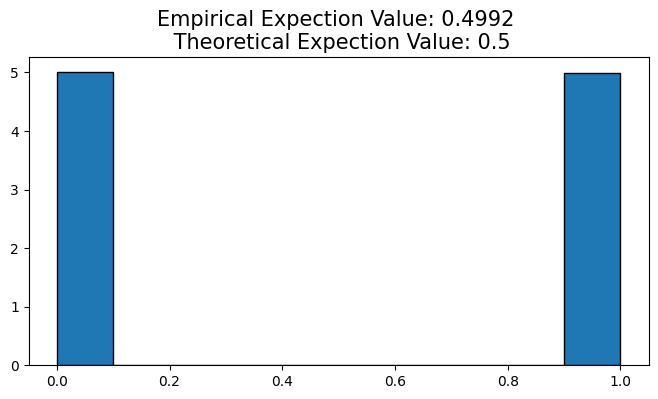
\includegraphics[width=0.6\textwidth]{ber_ITA.png}
		\caption{Inverse Transform method for generating  Bernoulli random numbers with $p=0.5$}
	\end{figure}
\end{example}

\begin{example}[Binomial Distribution]
	Let, $X\sim Bin(n,p)$ then,  $X$ has probability mass function
	\[
		f(r) = P(X=r) = {n\choose r}p^{r}(1-p)^{n-r},\  i = 1,2, \ldots
	\]
	The generation of $X\sim Bin(n,p)$ by Inverse Transform Algorithm can be tedious. We can use the relation between Binomial and Bernoulli distribution.
	If $x_i \sim Ber(p), \forall i = 1,2, \ldots, n$ then, $\sum_{i=1}^{n} x_i\sim Bin(n,p)$.

	Hence, by generating $x_i$ $n$ independent random variable from Bernoulli distribution and summing them we get binomial distribution
	\begin{figure}[H]
		\centering
		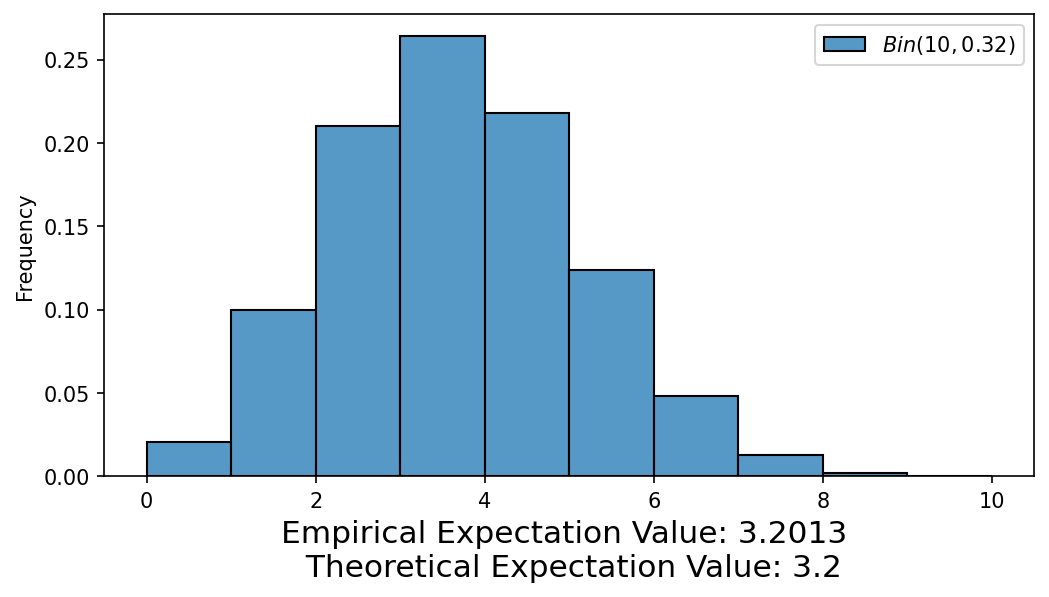
\includegraphics[width=0.6\textwidth]{images/bin_ITA.png}
		\caption{Generating  binomial random numbers with $n=10$ and  $p=0.32$}
	\end{figure}
\end{example}

\section{Generating Continuous Random Variables}

\subsection{The Inverse Transform Algorithm}
To generate Continuous random variables The Inverse Transform Algorithm is very important method. It is based on a following theorem.
\begin{theorem}
	\label{ITA theorem}
	Let $U$ be a uniform  $(0,1)$ random variable. For any continuous distribution function  $F$ the random variable  $X$ defined by
	\[
		X=F^{-1}(U)
	\]
	has distribution $F$.
\end{theorem}
\begin{proof}
	Let, $F_X$ denote the distribution function of  $X=F^{-1}(U)$. Then,
	\begin{align*}
		F_X(x) & = P(X\le x)         \\
		       & = P(F^{-1}(U)\le x) \\
	\end{align*}
	Since, $F$ is a cumulative distribution function it follows that $F(x)$ is monotonic increasing function of  $x$ and range of  $F(x)$ is  $(0,1)$.
	Then,
	\begin{align*}
		F_X(x) & = P\left(F\left(F^{-1}(U)\right)\le F(x)\right) \\
		       & = P(U\le F(x))                                  \\
		       & = F(x) \text{ since $U\sim U(0,1)$ }
	\end{align*}
\end{proof}

The above theory tells us we can generate a random variable $X$ from the continuous distribution function  $F$ by generating a random number $U\sim U(0,1)$
and setting $X=F^{-1}(U)$.

\begin{example}[Exponentian Distribution]
	\label{exponential distribution}
	Suppose we want to generate a random variable $x\sim Exp(\lambda)$, then its probability density function is
	\[
		f(x) = \lambda e^{-\lambda x}.
	\]
	Hence, The cumulative distribution function is,
	\[
		F(x) = 1-e^{\lambda x}
	\]
	if we let $x=F^{-1}(u)$, then,
	\begin{align*}
		u   & =F(x)=1-e^{-\lambda x}       \\
		1-u & = e ^{-\lambda x}            \\
		x   & = - \frac{\ln(1-u)}{\lambda}
	\end{align*}

	Hence, we can generate an exponential random variable with parameter 1 by generating a uniform $(0,1)$ random number $U$ and then setting
	\[
		X = F^{-1}(U) = -\frac{\ln(1-U)}{\lambda}.
	\]
	We see that if $U\sim U(0,1)$ then also $1-U\sim U(0,1)$ thus  $\ln(1-U)$ has the same distribution as  $\ln(U)$ so,
	\[
		X = F^{-1}(U) = -\frac{\ln(U)}{\lambda}.
	\]
	will also work. If we use second expression then the algorithm will take less computing power hence less time.
	\begin{figure}[H]

		\centering
		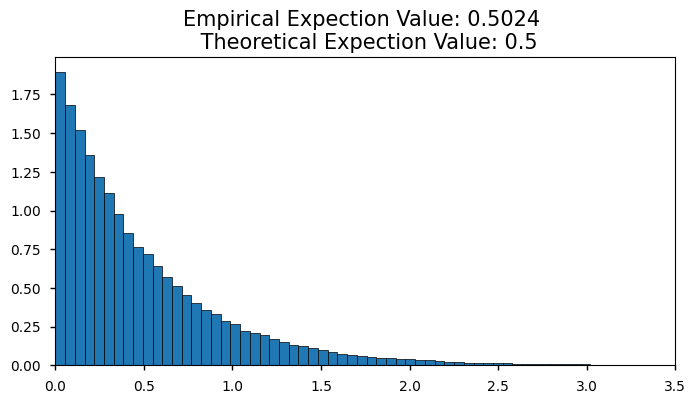
\includegraphics[width=0.6\textwidth]{images/exp_ITA.png}
		\caption{Inverse Transform method for generating $Exp(2)$}
	\end{figure}
\end{example}
\begin{example}[Gamma Distribution]
	Let $X\sim G(n,\lambda)$ Then, its probability  mass function is given by,
	\[
		f(x) = \frac{1}{\Gamma(n)}\lambda^{n}x^{n-1}e^{-\lambda x}
	\]

	We know if $X_i\sim Exp(\lambda) \forall i = 1,2, \ldots ,n$ then  $Y=\sum_i X_i \sim G(n,\lambda)$. As,

	\begin{align*}
		M_{Y}(t) = E \left[ e^{tY} \right] = E\left[ e^{\sum_{i=1}^{n} X_it  }\right] & = E\left[ \prod_{i=1}^{n} e^{X_it} \right]                                                \\
		                                                                              & =\prod_{i=1}^{n} E\left[  e^{X_it} \right] \text{ As all $X_i$ are independent }          \\
		                                                                              & = \prod_{i=1}^{n}\frac{\lambda}{\lambda-t} = \left( \frac{\lambda}{\lambda-t} \right)^{n}
	\end{align*}

	Then, Generating  $n$ number of $X_i\sim Exp(\lambda)$
	and summing them we can easily generate a random variable which follows gamma distribution
	\begin{figure}[H]

		\centering
		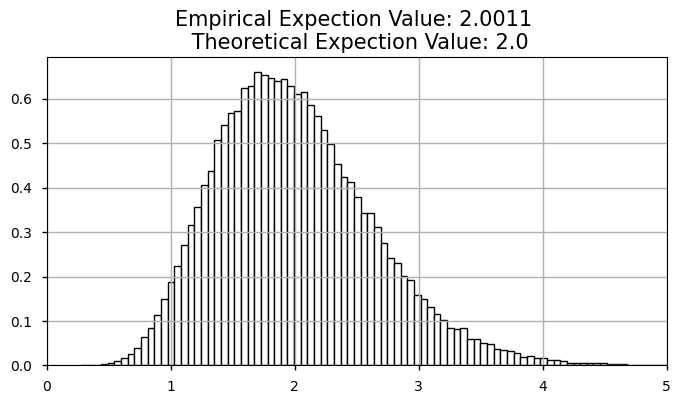
\includegraphics[width=0.6\textwidth]{images/gamma_ITA.png}
		\caption{$G(10,5)$ generated by summing of $Exp(5)$}
	\end{figure}
\end{example}

\subsection{Accept - Reject Method}
The accept–reject method is useful when it is difficult to directly simulate $f(x)$ but we can generate another density $g(x)$ such that $f(x)/g(x)$
is uniformly bounded and it is much easier to simulate $g(x)$. We simulate  $X$ from  $g$, and retain it or toss it according
to a probability proportional to $f(x)/g(x)$.
Because an $X$ value is either retained
or discarded, depending on whether it passes the admission rule, the method is called
the accept–reject method. The density $g(x)$ is called the envelope density.

The method proceeds as follows, \\
STEP 1: Find a density $g$ and a finite constant  $c$ such that  $\frac{f(x)}{g(x)}\le c \ \forall x$.\\
STEP 2: Generate $X\sim g$.\\
STEP 3: Generate  $U\sim U(0,1)$, independent of  $X$. \\
STEP 4: Retain this generated value  $X$ if  $U\le \frac{f(x)}{cg(x)}$.\\
STEP 5: Repeat the same until the required number of $n$ values of  $X$ has been obtained.\\

The following theorem supports the method.
\begin{theorem}
	Let $X\sim g$, and  $U$, independent of, be a distributed as $U[0,1]$. Then the conditional density of $X$ given that
	$U\le \frac{f(X)}{cg(X)}$ is $f$.
\end{theorem}
\begin{proof}
	Denote the CDF of $f$ by $F$. Then,
	\begin{align*}
		P\left( X\le x|U\le \frac{f(X)}{cg(X)} \right) & = \frac{P\left( X\le x, U\le \frac{f(X)}{cg(X)} \right)}{P\left( U\le \frac{f(x)}{cg(x)} \right)}                            \\
		                                               & = \frac{\int_{-\infty}^{x}\int_{0}^{\frac{f(t)}{cg(t)}}g(t)dudt}{\int_{-\infty}^{\infty}\int_0^{\frac{f(t)}{cg(t)}}g(t)dudt} \\
		                                               & = \frac{\int_{-\infty}^{x}f(t)dt}{\int_{-\infty}^{\infty}f(t)dt} = \frac{F(x)}{1}= F(x).
	\end{align*}
\end{proof}

\begin{example}[Generating a Normal Random Variable]
	\label{generate normal}
	To generate a standard normal variable $Z$ i.e. $Z\sim N(0,1)$, note first that the absolute value of  $Z$ has probability density function
	\begin{equation}
		\label{abs std normal}
		f(x) = \frac{2}{\sqrt{2\pi}}e^{- \frac{x^{2}}{2}} \ 0\le x \le \infty.
	\end{equation}
	Then, we can choose $g$ as the exponential density function with mean 1 i.e.
	\[
		g(x) = e^{-x}\ 0\le x\le \infty
	\]
	Now,
	\[
		\frac{f(x)}{g(x)} = \sqrt{\frac{2}{\pi}} e^{x-\frac{x^{2}}{2}}
	\]
	and so the maximum value of $f(x)/g(x)$ occurs at the value of $x$ that maximize $x-x^2 /2$ hence $x=1$ so we take
	\[
		c = \max_x \frac{f(x)}{g(x)} = \frac{f(1)}{g(1)} = \sqrt{\frac{2e}{\pi}}.
	\]
	Now,
	\[
		\frac{f(x)}{cg(x)} = \exp\left( x-\frac{x^2}{2}-\frac{1}{2} \right) = \exp\left( \frac{-(x-1)^2}{2} \right)
	\]
	Then, its follows that we can generate the absolute value of a standard normal random variable as follows: \\
	STEP 1: Generate $X\sim Exp(1)$. \\
	STEP 2: Generate $U\sim U(0,1)$, independent of $X$.\\
	STEP 3: If  $U\le \exp\left( -(X-1)^2 /2 \right)$, retain  $X$, Otherwise, return to Step 1.\\

	Once, we have simulated a random variable $X$ having density function as in
	Equation (\ref{abs std normal}) we can obtain a standard normal $Z$ by letting
	$Z$ be equally likely to be either  $X$ or  $-X$.
	In Step 3, the value $X$ is accepted if  $U\le \exp\left( -(X-1)^2 /2 \right)$, which is equivalent to $- \ln U\ge (X-1)^2 /2$.
	However, in Example (\ref{exponential distribution}) we have seen that $-\ln{U}\sim Exp(1)$ When $U\sim U(0,1)$.

	So, summing up, we can generate the standard normal random variable $Z$ as follows:\\
	STEP 1: Generate independent $X_1, X_2\sim Exp(1) $\\
	STEP 2: If $X_2\ge (X_1-1)^2 /2$ retain $X_1$. Otherwise, return to Step 1.\\
	STEP 3: Generate $U\sim U(0,1)$ and set,
	\begin{eqnarray*}
		Z=
		\begin{cases}
			X_1 \text{ if } U\le \frac{1}{2}, \\
			X_1 \text{ if } U> \frac{1}{2}.
		\end{cases}
	\end{eqnarray*}

	\begin{figure}[H]

		\centering
		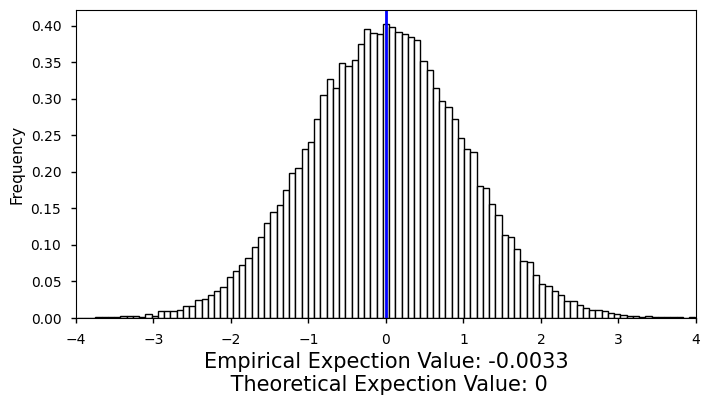
\includegraphics[width=0.6\textwidth]{images/nor_AR.png}
		\caption{Generating $N(0,1)$ with Accept - Reject method}
	\end{figure}

	If we want to generate normal random variable to have mean $\mu$  and variance $\sigma^2 $, just take $\mu +\sigma Z $.
\end{example}

\begin{example}[Generating Beta Distribution]
	\label{generate beta}
	If $\alpha$ and  $\beta $ are both getter then 1, then Beta density is uniformly bounded and its maximum attain at
	$\frac{\alpha-1}{\alpha+\beta-2}$. As a result the $U[0,1]$ density can be served as an envelope density for generating such Beta distribution by using accept-reject method.
	Precisely, generate $U$, $X\sim U[0,1]$ (independently), and retain the value if
	$U\le \frac{f(X)}{\sup_x f(X)}$, where,
	\[
		f(X)=\frac{\Gamma(\alpha+\beta)}{\Gamma(\alpha)\Gamma(\beta)}x^{\alpha-1} (1-x)^{\beta-1}, 0 < x< 1.
	\]
	Because
	\[
		\sup_x f(X) = f\left( \frac{\alpha-1}{\alpha+\beta-2} \right) = \frac{\Gamma(\alpha+\beta)}{\Gamma(\alpha)\Gamma(\beta)}\frac{(\alpha-1)^{\alpha-1} (\beta-1)^{\beta-1} }{(\alpha+\beta-2)^{\alpha+\beta-2} }
	\]
	The algorithm finally works out as follows:\\
	STEP 1: Generate independent $U,X \sim U[0,1]$.\\
	STEP 2: Retain the value $X$ if,
	\[
		U \le \frac{X^{\alpha-1} (1-X)^{\beta -1} (\alpha+\beta-2)^{\alpha+\beta-2} }{(\alpha-1)^{\alpha-1} (\beta-1)^{\beta-1} }.
	\]
	Otherwise, return to STEP 1.

	\begin{figure}[H]
		\centering
		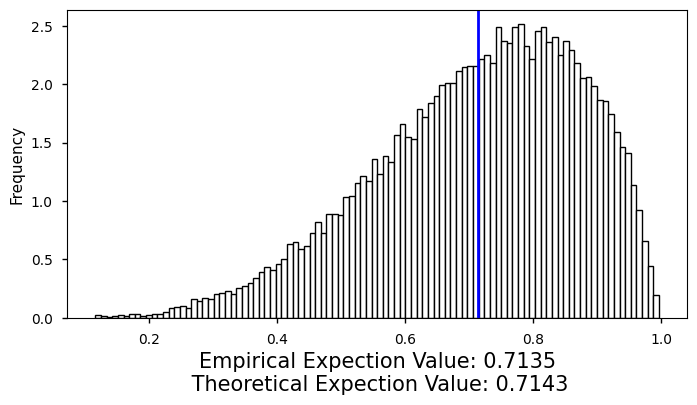
\includegraphics[width=0.6\textwidth]{images/beta_AR.png}
		\caption{Generating Beta(5,2) with accept-reject method}
		\label{Beta 5 2}
	\end{figure}
\end{example}

An issue about an accept-reject method is the acceptance rate.
Our goal make it as large as possible to increase the efficiency of the method.
This can be achieved by choosing $c$ to be smallest possible number, described in the result bellow.
\begin{theorem}[Acceptance Rate]
	For an accept-reject scheme, the probability that an $X\sim g$ is acceded is  $\frac{1}{c}$,
	and is maximized when $c$ is chosen to be $c=\sup_x\frac{f(x)}{g(x)}.$
\end{theorem}
\begin{proof}
	\begin{align*}
		P\left( U \le \frac{f(x)}{cg(x)} \right) & = \int_{-\infty}^{\infty} \int_{0}^{\frac{f(x)}{cg(x)}} g(t) du dt                                           \\
		                                         & = \int_{-\infty}^{\infty} \frac{f(t)}{cg(t)}g(t)dt = \int_{-\infty}^{\infty} \frac{f(t)}{c}dt = \frac{1}{c}.
	\end{align*}
	Because any $c$ that can be chosen must be at least as large as $\sup_x\frac{f(x)}{g(x)}$
	, obviously $1/c$ is maximized by choosing $c=\sup_x\frac{f(x)}{g(x)}.$
\end{proof}

In the example (\ref{generate normal}) for $N(0,1)$ the acceptance rate is $\sqrt{\frac{\pi}{2 e}} = 0.7601$.
And for example (\ref{generate beta}) for Beta(5,2) the acceptance rate is 0.4069

\subsection{Bivariate Techniques}
Let $X$ and $Y$ be independent slandered normal random variable and let $R$ and $\theta$
denote the polar coordinates of vector $(X,Y)$. That is,
\begin{align*}
	R^{2}       & = X^{2} + Y^2 \\
	\tan \theta & = \frac{Y}{X}
\end{align*}

Since $X$ and $Y$ are independent, their joint density is the product of their individual densities and thus given by
\begin{align*}
	f(x,y) & = \frac{1}{\sqrt{2\pi}} e^{-x^{2}/2 } \frac{1}{\sqrt{2\pi}} e^{-y^{2}/2 } \\
	       & = \frac{1}{2\pi} e^{-(x^{2}+y^{2})/2}
\end{align*}
To determine the joint density of $R^{2} $ and $\Theta$ - call it $g(d,\theta)$ we make the change of variables
\[
	d=x^{2}+y^{2}, \ \  \theta=\tan^{-1}\left( \frac{y}{x} \right)
\]
Then the joint density function of $d $ and $\Theta$ is,

\begin{align*}
    \label{jacobian transformation}
    g(d,\theta) &= |J| f(x,y) \\ 
                &= |J| \frac{1}{2\pi} e^{-(x^{2}+y^{2})/2} \numberthis
\end{align*}
where,
\[
	J =
	\begin{vmatrix}
        \frac{\partial x}{\partial t} & \frac{\partial x}{\partial \theta} \\[1ex]
		\frac{\partial y}{\partial t} & \frac{\partial y}{\partial \theta} \\
	\end{vmatrix} = \frac{1}{2}.
\]
Then, replacing the value of $ x = \sqrt{d}\sin(\theta)  $ and $ y=\sqrt{d}\cos(\theta) $ in the Equitation (\ref{jacobian transformation}) we get,
\begin{equation}
	g(d,\theta) = \frac{1}{2}\frac{1}{2\pi} e^{-d/2},\ \ \ 0< d<\infty, 0<\theta<2 \pi.
\end{equation}

As $g(d,\theta)$ is equal to product of the product of $Exp(1/2)$ density and $U(0,2 \pi)$, it follows that,\\
$R^{2}$ and $\Theta$ are independent, with $R^{2} \sim Exp(1/2)$ and $\Theta \sim U(0, 2 \pi)$ \\
Hence to generate a pair of independent slandered normal random variables $X$ and $Y$ by generating $R^{2} $ and $\Theta$ in polar coordinates and then
transform back to rectangular coordinates. Hence the algorithm is:\\
STEP 1: Generate random number $U_1, U_2 \sim U(0,1)$.\\
STEP 2: $ R^{2} = - 2 \ln U_1 $ and $\Theta = 2 \pi U_2 $. \\
STEP 3: Now let,
\begin{align*}
	X & = R \cos \Theta = \sqrt{-2\ln U_1}\cos(2 \pi U_2)                                   \\
	Y & = R \sin \Theta = \sqrt{-2 \ln U_1} \sin(2 \pi U_2). \label{Box-muller} \numberthis
\end{align*}

The transformation given by equitations (\ref{Box-muller}) are known as Box-Muller transformation.

\begin{figure}[H]
	\centering
	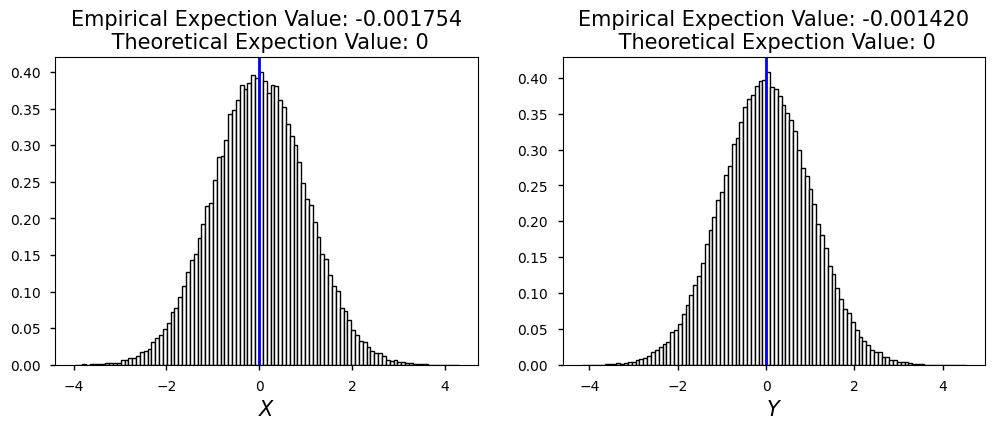
\includegraphics[width=0.9\textwidth]{images/nor_polar.png}
	\caption{Generating independent $X, Y \sim N(0,1)$ with polar method}
	\label{normal polar}
\end{figure}


\chapter{Ordinary Monte Carlo Simulation}
Polish-American mathematician Stanislaw Ulam, recovering from an illness, was playing a lot of
solitary card game. He wanted to calculate the probability of winning and
quickly it is impossible to calculate analytically. Then he thought about playing
lots of hands counting number of wins, but decided it will take years.
After falling several times he asked Von Neumann to build a program to simulate solitary
card game in ENIAC. Then Around 1940 they used Monte Carlo simulation in Manhattan Project
in which physicists wanted to understand how the physical
properties of neutrons would be affected by various possible scenarios following a
collision with a nucleus.

The basis for Monte Carlo is Law of Large Number. If we simulate large number $X_1, X_2, \ldots$ iid
copes of random variable $X$ Then we can approximate the true value $E(f(X))$ by simple mean
$\frac{1}{n}\sum_{i=1}^{n} f(X_i)$. Here in Monte Carlo Random Sampling play the key factor for good estimation of $E(f(X))$.

\section{Evaluate Integrals using Monte Carlo simulation}
The application of Monte Carlo is to computation of integrals. Let $g(x)$ be a function
and suppose we wanted to compute $I$ where
\[
	I = \int_{0}^{1} g(x) dx
\]

To compute the value of $I$, note that if $U\sim U[0,1]$ then we can express $I$ as
\[
	I = E[g(U)]
\]
If $U_1, \ldots, U_n$ are independent uniform $(0,1)$ random variables, it thus follows that
the random variables $g(U_1),\ldots,g(U_n)$ are independent and identically distributed random
variable having mean $I$. Therefore, by law of large numbers, its follows that,
with probability,
\[
	\sum_{i = 0}^{n} \frac{g(U_i)}{n} \to E(g(U))= I \text{ as } k \to \infty
\]

Hence we can approximate $I$ by generating a large number of random numbers $U_i$ and taking
as our approximation the average value of $g(U_i)$.

If we wanted to compute
\[
	I = \int_{a}^{b} g(x) dx
\]
then , by taking the substitute $y=(x-a)/(b-a)$, $dy = dx/(b-a)$, we see that
\begin{align*}
	I & = \int_{0}^{1} g(a+[b-a]y)(b-a)dy \\
	  & = \int_{ 0}^{1} h(y) dy
\end{align*}

Where $h(y)= (b-a)g(a+[b-a]y)$. Thus we can approximate $I$ by continually generating random
numbers and then taking the average value of $h$ evaluated at these random numbers.

Similarly, if we wanted
\[
	I = \int_{0}^{\infty} g(x) dx
\]

we could apply the substitution $y=1/(x+1)$, $dy=-dx/(x+1)^{2} = -y ^{2} dx$, to obtain the identity
\[
	I=\int_{0}^{1} h(y)dy
\]
where, \[
	h(y) = \frac{g(\frac{1}{y} -1)}{y ^{2}}
\]
Using this technique we can also evaluate multidimensional integrals. Suppose that $g$ is a function with n-dimention argument
and we are interested in computing
\[
	I = \int_{0}^{1} \int_{0}^{1} \ldots \int_{0}^{1} g(x_1, x_2 , \ldots , x_n) dx_1 dx_2 \ldots dx_2.
\]
Then, we can express $I$ as
\[
	I = E(g(U_1, U_2, \ldots U_n))
\]
where $U_1, U_2, \ldots U_n \sim U[0,1]$  Hence  if we generate $k$ independent sets, each consisting of $n$ independent $U[0,1]$
random variable
\begin{align*}
	U_1^{1}   & \ldots U_n^{1}  \\
	U_1^{2}   & \ldots U_n^{2}  \\
	          & \vdots          \\
	U_1^{k} , & \ldots, U_n^{k}
\end{align*}
then, since the random variables $g(U_1^{i},\ldots, U_n^{i}), i = 1,2,\ldots,k  $ are all independent and identically distributed
random variable with mean $I$, we can estimate $I$ by $\sum_{i = 1}^{k}g(U_1^{i} , \ldots, U_n^{i} )/k $.

\begin{example}
	Suppose we want to integrate,
	\[
		I = \int_{0}^{1} e^{-\frac{x ^{2}}{2}} dx.
	\]

	Then we can say that,
	\[
		I = E(e^{-\frac{U ^{2}}{2}})
	\]
	where, $U\sim U[0,1]$. Then simulating a large number of $U_1, U_2, \ldots, U_n\sim U[0,1]$ and calculating,
	\[
		\sum_{i = 1}^{n}  \frac{e^{-\frac{U_i ^{2}}{2}}}{n}
	\]
	we can evaluate $I$.

	Hence the algorithm is:\\
	STEP 1: Generate $U\sim U[0,1]$. \\
	STEP 2: Calculate $ e^{-\frac{U ^{2}}{2}} $ and retain it. goto STEP 1. \\
	STEP 3: After large number of iteration evaluate the average.
	\begin{table}[H]
		\begin{center}
			\begin{tabular}{l c}
				\hline
				Monte Carlo sample size & Monte Carlo Estimate of I = 0.8556 \\
				\hline
				50                      & 0.8555                              \\
				100                     & 0.8558                              \\
				1000                    & 0.8555                              \\
				10000                   & 0.8556                              \\
				100000                  & 0.8556                              \\
				\hline
			\end{tabular}
			\caption{Monte Carlo Integration of $e^{-x ^{2}/2}$.}
		\end{center}
	\end{table}
	\begin{figure}[H]
		\centering
		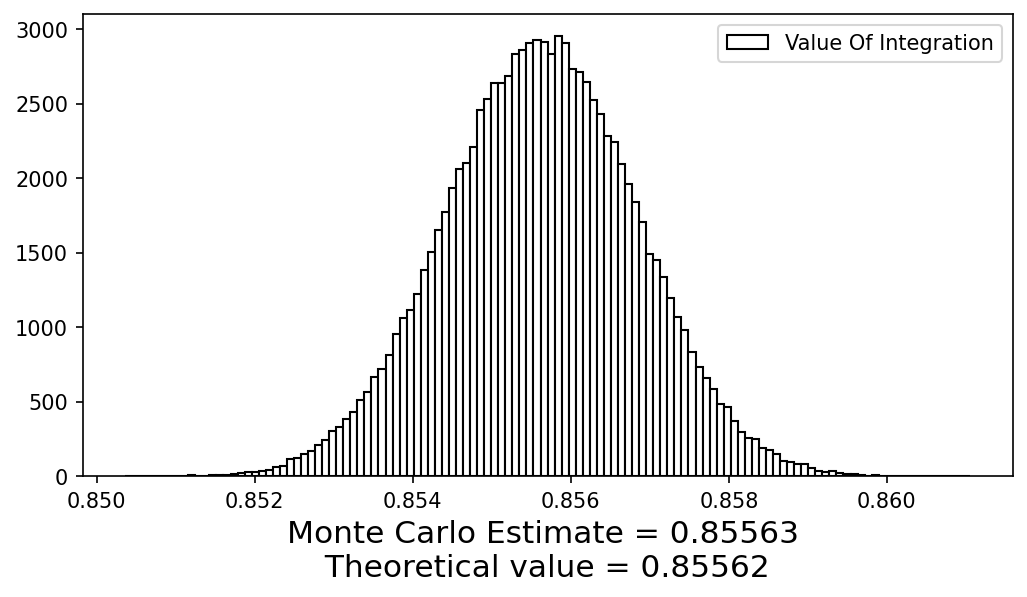
\includegraphics[width=0.6\textwidth]{images/evaluating_integration.png}
		\caption{Monte Carlo Integration of $e^{-x ^{2}/2} $}
	\end{figure}
	Here, we see by the time the Monte Carlo sample size is 100000, we get fairly
	accurate estimates for the value $I$.
\end{example}

\section{The Estimation of $\pi$}
Suppose that the random vector $(X,Y)$ is uniformly distribution in the square of area 4
centered at the origin. That is, it is a random point in the region specified in Figure \ref{Square}.
Let us consider now the probability that this random point in the square in contained within the inscribed circle of radius 1
like the Figure \ref{Circle within Square}.

\begin{figure}[H]
	\centering
	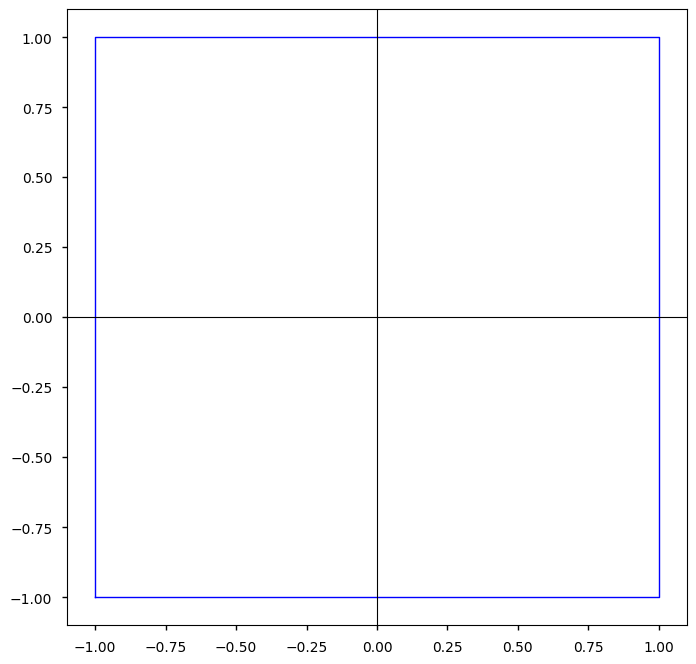
\includegraphics[width=0.4\textwidth]{images/square.png}
	\caption{Square}
	\label{Square}
\end{figure}

\begin{figure}[H]
	\centering
	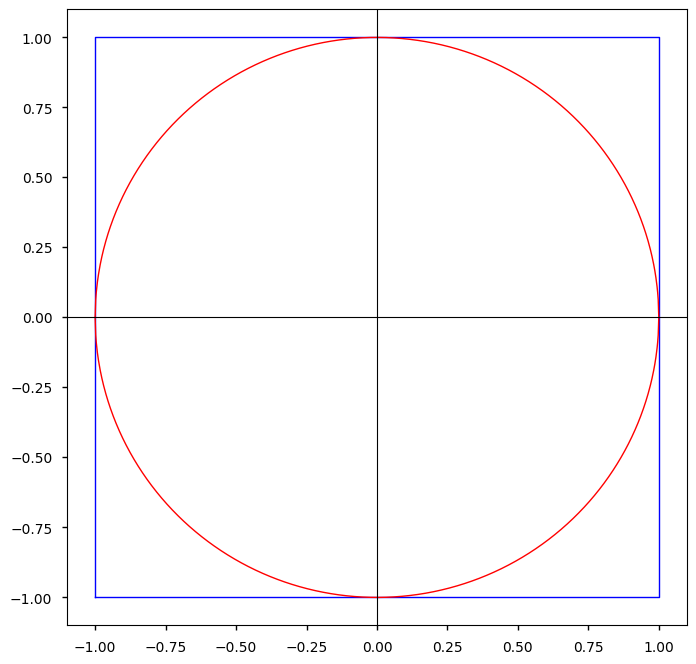
\includegraphics[width=0.4\textwidth]{images/circle.png}
	\caption{Circle within Square}
	\label{Circle within Square}
\end{figure}

Note that since $(X,Y)$ is uniformly distributed in the square it follows that
\begin{align*}
	P((X,Y) \text{ is in the circle } ) & = P(X ^{2}+ Y ^{2}\le 1)                                                        \\
	                                    & = \frac{\text{Area of the circle} }{\text{Area of the square} } = \frac{\pi}{4}
\end{align*}

Hence we generate a large number of points in the square, the proportion of points that fall within the circle will be approximately $\pi/4$.
Now, if $X$ and $Y$ were independent and both were uniformly distributed over $(-1,1)$, their joint density would be
\begin{align*}
	f(x,y) & = f(x)f(y)                                         \\
	       & = \frac{1}{2} \times \frac{1}{2}                   \\
	       & = \frac{1}{4} , \  -1 \le x \le 1,\ -1 \le y \le 1
\end{align*}

Since, the density function of $(X,Y)$ is constant in the square, it thus follows that $(X,Y)$ is uniformly distributed in the square.
Now, if $U\sim U[0,1]$ then $2U\sim U[0,2]$ and so $2U-1\sim U[-1,1]$. Therefore, if we generate ranom numbers $U_1 \text{ and }  U_2$
and set $X=2U_1 - 1$ and $Y= 2U_2-1$, and define,
\[
	I = \begin{cases}
		1 \text{ if } X ^{2} + y ^{2} \le 1 \\
		0 \text{ otherwise }
	\end{cases}
\]
Then,
\[
	E(I)=P(X ^{2} + y ^{2} \le 1) = \frac{\pi}{4}.
\]
Hence the Algorithm for estimating $\pi$ is:\\
STEP 1: Set Circle = 1. \\
STEP 2: Generate $U_1, U_2\sim U[0,1]$\\
STEP 3: If $(2U_1-1)^{2}+ (2U_2-1)^{2} \le 1$ Set Circle = Circle + 1, Otherwise return to STEP 2.
STEP 4: After simulating $N$ time, set $\text{Area of Circle}  = \text{Circle}  / N$

\begin{table}[H]
	\centering
	\begin{tabular}{l c}
		\hline
		Monte Carlo sample & Monte Carlo Estimate of $\pi$ \\
		\hline
		50                 & 2.9600                        \\
		100                & 3.0800                        \\
		1000               & 3.1200                        \\
		10000              & 3.1428                        \\
		100000             & 3.1397                        \\
		1000000            & 3.1394                        \\
		10000000           & 3.1414                        \\
		\hline
	\end{tabular}
	\caption{Monte Carlo Estimates of $\pi$}
	\label{tab:montecarlopi}
\end{table}
Here, we see by the time the Monte Carlo sample size is 10000000, we get fairly accurate estimates for $\pi$



\section{Importance Sampling}
There are two different ways to think about importance sampling.
The more traditional one is to go back to the primary problem that
Monte Carlo  wants to solve,
namely to approximate the value of an expectation
$\mu = \int \phi_0(x)dF_0(x) $ for some function $\phi_0$ and some CDF $F_0$.
However, $(\phi_0,F_0)$ is not the only pair $(\phi,F)$ for which
$\int \phi(x)dF(x) $ equals the specific number $\mu$. Indeed, given any other
CDF $F_1$,
\begin{align*}
	\mu & = \int \phi_0(x)dF_0(x)                      \\
	    & = \int \phi_0(x)\frac{dF_0}{dF_1}(x) dF_1(x) \\
	    & = \int \lambda(x)\phi_0(x)dF_1(x).
\end{align*}

where $\lambda(x)=\frac{dF_0}{dF_1}(x)$. If $F_0$, $F_1$ have densities
$f_0$, $f_1$, then $\lambda(x)=\frac{f_0(x)}{f_1(x)}$; if $F_0,$ $F_1$
have respective pmfs $f_0$, $f_1$, then also $\lambda(x)=\frac{f_0(x)}{f_1(x)}$
This raises the interesting possibility that we can sample from a general $F_1$, and
subsequently use the usual Monte Carlo estimate
\[
	\hat{\mu} = \frac{1}{n} \sum_{i = 1}^{n} \lambda(X_i)\phi_0(X_i) = E_{F_1}[\lambda(X_i)\phi_0(X_i)].
\]

where $X_1, X_2, \ldots, X_n$ is Monte Carlo sample from $F_1$.
Importance sampling poses the problem of finding an optimal choice of $F_1$ for which to sample,
so that $\hat{\mu}$ has the smallest possible variance.
The distribution $F_1$ hat ultimately gets
chosen is called the \textit{importance sampling distribution}.

We can visualize this method by an example.

\begin{example}
	\label{ex:reductionofvariance}
	Suppose we want to evaluate
	\[
		I = \int_{0}^{10} e^{-2 |x-5|} dx.
	\]
	doing it analytically we get $I = 0.9999$.

	Now, suppose $\phi(x) = e^{-2 |x-5|}$ then we want to evaluate
	\[
		I = \int_{0}^{10} \phi(x) dx
	\]
	Now,
	\begin{align*}
		\label{hx with U}
		I & = \int_{0}^{10} \phi(x) dx                                                                                                            \\
		  & = \int_{0}^{10} \phi(x)\frac{10}{10} dx                                                                                               \\
		  & = \int_{0}^{10} 10 \times \phi(x) \frac{1}{10} dx = \int_{0}^{10} 10\phi(x) f_0(x) dx \text{ where } f_0(x)\text{ pdf of }U(0,1) \numberthis \\
		  & = E_U[10 \times \phi(U)] \text{ where, }  U\sim U(0,10).
	\end{align*}

	By Ordinary Monte Carlo technique we can estimate $I$ by $\frac{1}{N}\sum_{i = 1}^{N} 10 \times \phi(U_i)$ where $U_i\sim U(0,10)$ for $i=1,2,\ldots,N$
	for the large number of $N$.
	\begin{figure}[H]
		\centering
		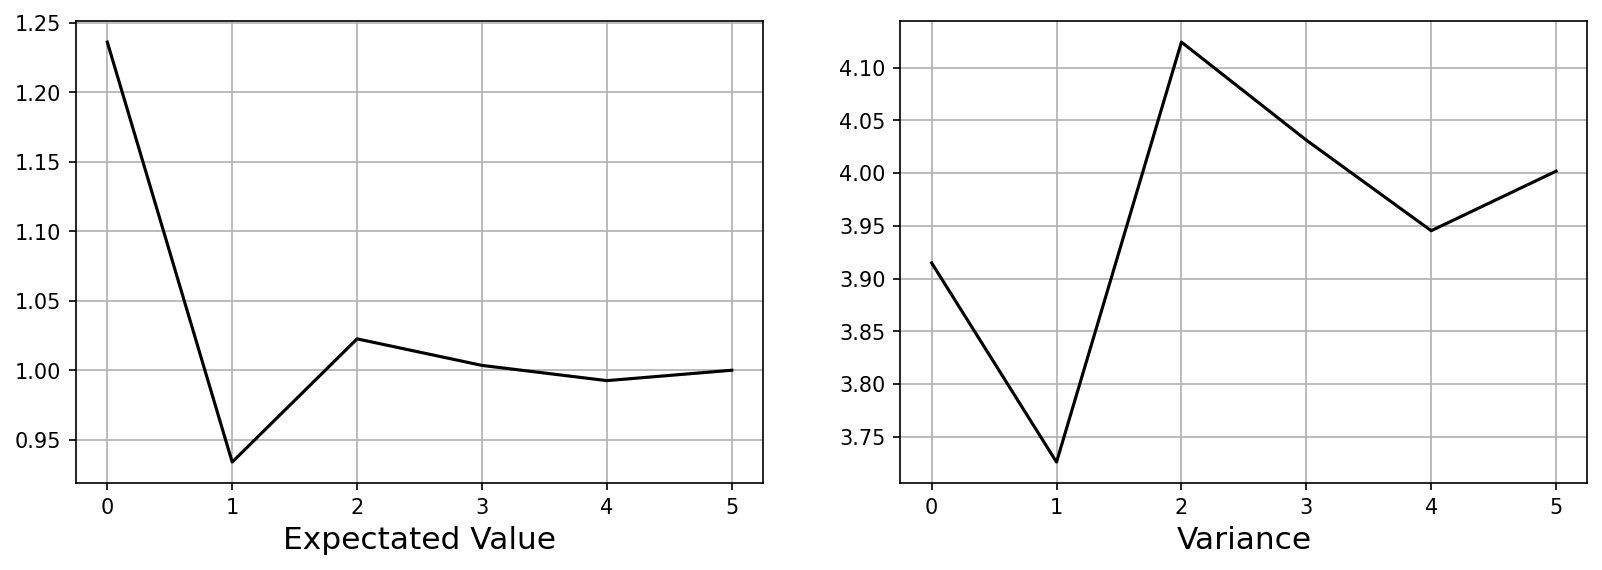
\includegraphics[width=0.8\textwidth]{int_h(x)_MC.png}
		\caption{Monte Carlo integration of $\int_{0}^{10} e^{-2 |x-5|} dx$.}
		\label{MC:IntegrationOFe-2|x*5|}
	\end{figure}
	\begin{table}[h]
		\centering
		\begin{tabular}{lcc}
			\hline
			Sample Size & Estimated Value I=0.9999 & Variance \\
			\hline
			10          & 2.3243                   & 5.6912   \\
			100         & 1.0372                   & 3.6717   \\
			1000        & 0.8871                   & 3.5543   \\
			10000       & 1.0467                   & 4.2416   \\
			100000      & 1.0053                   & 4.0089   \\
			1000000     & 1.0054                   & 4.0346   \\
			\hline
		\end{tabular}
		\caption{Monte Carlo integration of $\int_{0}^{10} e^{-2 |x-5|} dx$.}
		\label{tab:IntegrationOFe-2|x*5|}
	\end{table}
	Here we can see that for sample size 1M, we get a pretty good estimation of $I$ with less then $0.6\%$ error. But the variance is very high.
	If we see at left of \Cref{fig:hxwithU01andN01} we can see we are taking unnecessary value from low frequency part of $\phi(x)$ that is,
	from extreme left and right. If we choose an importance sampling distribution that has similar curve as $\phi(x)$, then we can estimate $I$ with low variance.
	If we choose importance sampling distribution as $N(5,1)$ then we see from right of \Cref{fig:hxwithU01andN01} it has similar pattern as $\phi(x)$.
	\begin{figure}[H]
		\centering
		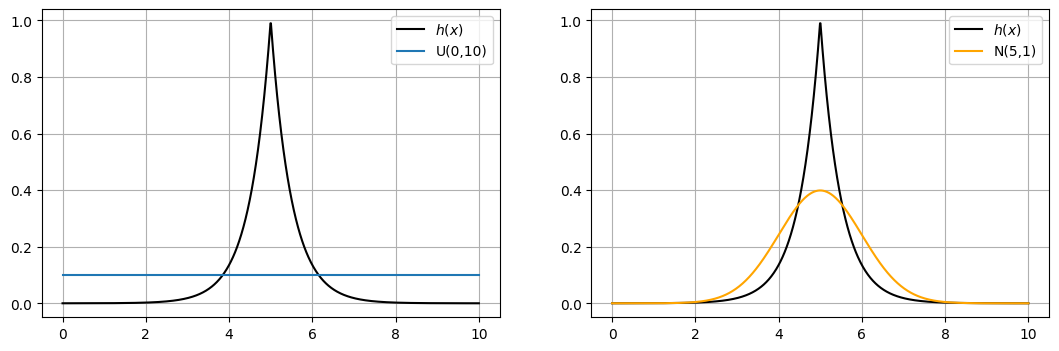
\includegraphics[width=0.8\textwidth]{h(x)_with_normal_and_uniform.png}
		\caption{$h(x)$ with $U(0,10)$ and $N(5,1)$}
		\label{fig:hxwithU01andN01}
	\end{figure}

	Let, $f_1(x)$ is pdf of $N(0,1)$ then, from \Cref{hx with U}
	\begin{align*}
		I & = \int_{0}^{10} 10\phi(x) f_0(x) dx                                            \\
		  & = \int_{0}^{10} 10 \phi(x) \frac{f_0(x)}{f_1(x)} q(x)dx                          \\
		  & = E_X\left[ 10 \phi(X) \frac{f_0(X)}{f_1(X)} \right] \text{ where } X\sim N(5,1) \\
		  & = E_X\left[ 10 \phi(X) \lambda(X) \right]\text{ where } X\sim N(5,1)
	\end{align*}
	Where, $\lambda(x) = \frac{f_0(x)}{f_1(x)}$ here $f_0(x)$ is pdf of $U(0,1)$ and $f_1(x)$ is pdf of $N(5,1)$. Now using usual Monte Carlo estimate
	\[
		I = \frac{1}{N} \sum_{i = 1}^{N} 10 \phi(X_i) \lambda(X_i)
	\]
	where $X_1, X_2,\ldots,X_N$ is Monte Carlo sample from $N(5,1)$.
	\begin{table}[H]
		\centering
		\begin{tabular}{l c c}
			\hline
			Sample Size & Estimated Value (I=0.9999) & Variance \\
			\hline
			10          & 1.2473                     & 0.3812   \\
			100         & 0.9292                     & 0.2593   \\
			1000        & 1.0018                     & 0.3550   \\
			10000       & 1.0072                     & 0.3603   \\
			100000      & 1.0039                     & 0.3595   \\
			1000000     & 0.9999                     & 0.3580   \\
			\hline
		\end{tabular}
		\caption{Evaluating $\int_{0}^{10} e^{-2 |x-5|} dx$ using Importance Sampling.}
		\label{tab:mytable}
	\end{table}
	
	\begin{figure}[H]
		\centering
		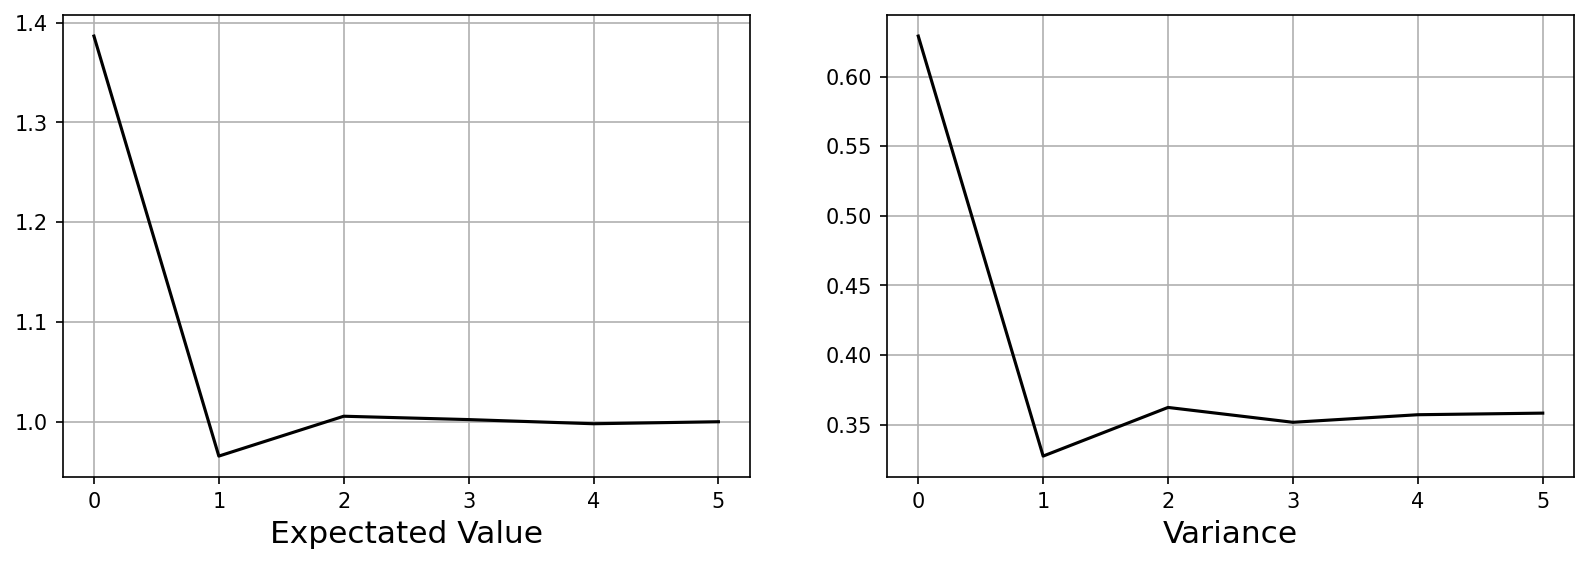
\includegraphics[width=0.8\textwidth]{int_h(x)_ipsam.png}
		\caption{Evaluating $\int_{0}^{10} e^{-2 |x-5|} dx$ using Importance Sampling.}
		\label{fig:impotrancesampling1}
	\end{figure}
	Here we can see that the estimation of $I$ is pretty close and variance is also
	lower the Original Monte Carlo method.
\end{example}

A more contemporary view of importance sampling is that we do not approach
importance sampling as an optimization problem, but because the circumstances
force us to consider different sampling distributions $F$.

Now, we also assume that $F_0,$ $F_1$ both have densities, say $f_0$, $f_1$.
If $F_0$, $F_1$ are both discrete then the notation only change but the argument is same.
Suppose then $f_i(x)=\frac{h_i(x)}{c_i},\ i=0,1$, where the assumption is that $h_0$, $h_1$
are completely known and also computable, but $c_0$, $c_1$ are unknown and are not even computable.
Then, as we showed above, for any function $\phi$ for which the expectation $E_{F_0}[\phi(X)]$ exist,

\begin{align*}
	\mu & = E_{F_0}[\phi(X)] := \int \frac{f_0(x)}{f_1(x)}\phi(x)f_1(x)dx      \\
	    & =\frac{c_1}{c_0} \int \frac{\phi(x)h_0(x)}{h_1(x)}f_1(x)dx           \\
	    & =\frac{c_1}{c_0} E_{F_1}\left( \frac{\phi(X)h_0(X)}{h_1(X)} \right).
\end{align*}

This is a useful reduction, but we have to deal with the fact that ratio $\frac{c_1}{c_0}$
is not known to us. Now, if we use the special function $\phi(x)\equiv 1$, the same
representation above gives us
\begin{align*}
	1                        & = \frac{c_1}{c_0} E_{F_1} \left( \frac{h_0(X)}{h_1(X)} \right) \\
	\implies \frac{c_1}{c_0} & = \frac{1}{E_{F_1} \left( \frac{h_0(X)}{h_1(X)} \right)}
\end{align*}
and because $h_0,$ $h_1$ are explicitly known to us, we have a way to get rid of the
quotient $\frac{c_1}{c_0}$ and write the final \textit{importance sampling identity}
\begin{align*}
	E_{F_0}[\phi(x)] = \frac{E_{F_1}\left( \frac{\phi(X)h_0(X)}{h_1(X)} \right)}{E_{F_1} \left( \frac{h_0(X)}{h_1(X)} \right)}
\end{align*}
We can now use an available Monte Carlo sample $X_1,X_2,\ldots,X_n$ from $F_1$
to find Monte Carlo estimates for $\mu = E_{F_0}[\phi(x)]$

The basic plug-in estimate for $\mu$ is the so-called ratio estimate
\[
	\hat{\mu} = \frac{\sum_{i = 1}^{n}\frac{\phi(X_i)h_0(X_i)}{h_1(X_i)} }{\sum_{i = 1}^{n} \frac{h_0(X_i)}{h_1(X_i)}}.
\]

\begin{example}[Binomial Bayes problem with an Atypical Prior]
	\label{Binomial Bayes problem with an Atypical Prior}
	Suppose $X\sim Bin(m,p)$ for some fixed $m$ and $p$ has the prior density $c\sin^{2}(\pi p)$,
	where $c$ is a normalizing constant.
	Throughout the example, $c$ denotes a generic constant,
	and is not intended to mean the same constant at every use.

	The posterior density of $p$ given $X = x$ is
	\[
		\pi(p|X=x) = cp^{x}(1-p)^{m-x}\sin ^{2}(\pi p), \ \ 0<p<1.
	\]
	The problem is to find the posterior mean
	\[
		\mu = c \int_{0}^{1} p[cp^{x}(1-p)^{m-x}\sin ^{2}(\pi p)]dp.
	\]

	We use importance sampling to approximate the value of $\mu$. Towards this, choose
	\[
		\phi(p)=p, \ h_0(p) = p^{x} (1-p)^{m-x} \sin ^{2}(\pi p),\ h_1(p) = p^{x}(1-p)^{m-x},
	\]
	so that if $p_1,p_2,\ldots,p_n$ are samples from $F_1$, (i.e. $p_i\sim Beta(x+1, m-x+1)$),
	then the importance sampling estimate of the posterior mean $\mu$ is
	\begin{align*}
		\hat{\mu} & = \frac{\sum_{i=1}^{n}\frac{\phi(p_i)h_0(p_i)}{h_1(p_i)} }{\sum_{i=1}^{n}\frac{h_0(p_i)}{h_1(p_i)} } \\
		          & = \frac{\sum_{i=1}^{n}p_i\sin ^{2}(\pi p_i) }{\sum_{i=1}^{n} \sin ^{2}(\pi p_i) }.
	\end{align*}

	Note that we did not need to calculate the normalizing constant in the posterior density.
	We take $m=100$, $x=45$ for specificity.
	\begin{table}[H]
		\centering
		\begin{tabular}{l p{4.5cm} p{2cm}}
			\hline
			Sample Size & Importance Sampling Estimate of $\mu$ & Variance \\
			\hline
			20          & 0.4821                                & 0.5465   \\
			50          & 0.4629                                & 0.5162   \\
			100         & 0.4597                                & 0.4929   \\
			250         & 0.4635                                & 0.4902   \\
			500         & 0.4585                                & 0.4962   \\
			\hline
		\end{tabular}
		\caption{Importance Sampling Estimates of $\mu$ for Different Sample Sizes}
		\label{tab:importance-sampling-mu}
	\end{table}
    \begin{figure}[H]
        \centering
        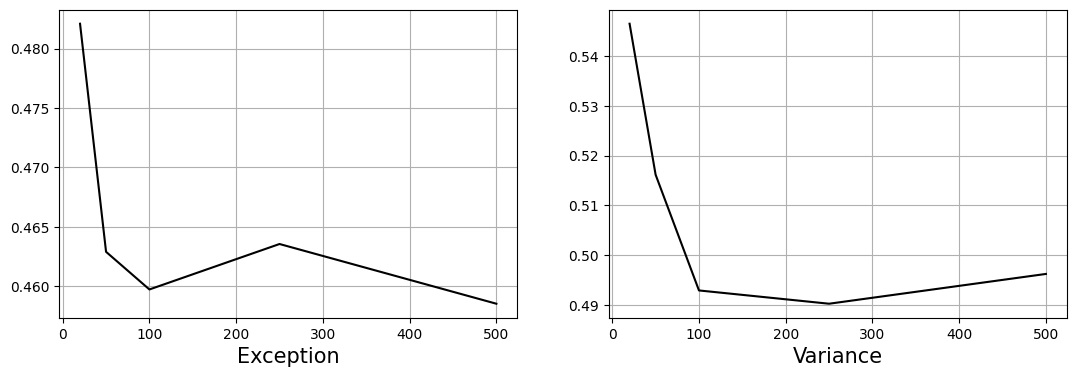
\includegraphics[width=0.8\textwidth]{chap4ex2.png}
        \caption{Exception and variance graph of Binomial Bayes problem with an Atypical Prior}
    \end{figure}
\end{example}

\subsection{Optimal Importance Sampling Distribution}
We now address the question of the optimal choice of the importance sampling
distribution. There is no unique way to define what an optimal choice means. We
formulate one definition of optimality and provide an optimal importance sampling
distribution. The optimal choice would not be practically usable, as we shown.
However, the solution still gives useful insight.

\begin{theorem}
	Consider the importance sampling estimator $\hat{\mu} = \frac{1}{n}\sum_{i=1}^{n} \lambda(X_i)\phi(X_i) $ for $\mu=\int \phi(x)f_0(x)dx $, where
	$\lambda(x) =\frac{f_0(x)}{f_1(x)}$, and $X_1,\ldots,X_n$ are iid observations from $F_1$
	Assume that $\phi(x)\ge0$, and $\mu>0$. Then, $Var_{F_1}(\hat{\mu})$ is
	minimized when $f_1(x)=\frac{\phi(x)f_0(x)}{\mu}$.
\end{theorem}
\begin{proof}
	Because $X_1,\ldots,X_n$ is iid, so are $\lambda(X_1)\phi(X_1),\ldots,\lambda(X_n)\phi(X_n)$, and hence,
	\[
		Var_{F_1}(\hat{\mu}) = \frac{1}{n} Var_{F_1}(\lambda(X_1)\phi(X_1))
		.
	\]

	Clearly, this is minimized when with probability one under $F_1$, $\lambda(X_1)\phi(X_1)$
	is constant, say $k$. The constant $k$ must be equal to the mean of $\lambda(X_1)\phi(X_1)$, that is,
	\begin{align*}
		k & = \int \lambda(x)\phi(x)f_1(x)dx              \\
		  & = \int \frac{\phi(x)f_0(x)}{f_1(x)} f_1(x) dx \\
		  & = \int \phi(x)f_0(x)dx = \mu.
	\end{align*}
	Therefore, the optimal importance sampling density satisfies $\lambda(x)\phi(x) = \mu$
	hence,
	\[
		f_1(x) = \frac{\phi(x)f_0(x)}{\mu}.
	\]
\end{proof}
This is not usable in practice, because it involves $\mu$,which is precisely the unknown number we want to approximate.
However, the theoretically optimal solution
suggests that the importance sampling density should follow key properties of the
unnormalized function $\phi(x)f_0(x)$.
For example, $f_1$ should have the same shape and tail behavior as $\phi(x)f_0(x)$.

We have seen this phenomena in the \Cref{Binomial Bayes problem with an Atypical Prior}.
Because Graph of $\phi(x)h_0(x)$ and $h_1(x)$ in \Cref{fig:ch4ex2plothx}, they both have the same key properties.   
\begin{figure}[H]
    \centering
    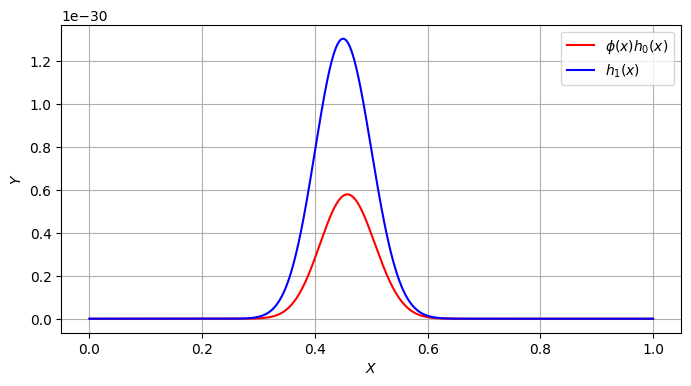
\includegraphics[width=0.6\textwidth]{ch4ex2plot_hx.png}
    \caption{Graph of $\phi(x)h_0(x)$ and $h_1(x)$}
    \label{fig:ch4ex2plothx}
\end{figure}

\chapter{Markov Chain Monte Carlo Methods}

\textit{Markov Chain Monte Carlo}(MCMC) is a powerful collection of algorithms that enable us to simulate from complicated distributions using Markov chains. 
When the target distributions is an unconventional one, or it is known only up to a normalizing constant that is $ f(x) = \frac{h(x)}{c} $ for some explicit function $ h $ but only an implicit normalizing constant $ c $, because $ c $ can not be computed exactly, the standard simulation techniques are difficult to apply or even not applicable in that case \textit{Markov Chain Monte Carlo}(MCMC) comes in to play.
The basic idea for MCMC is to construct a \textit{Markov Chain} whose stationary distribution is the distribution of interest.

MCMC is widely used algorithms it is primarily used for calculating numerical approximations  of multi-dimensional integration for example is Bayesian statistic, computational physics, computational biology.
In Bayesian statistic, Markov Chain Monte Carlo method are typically used to calculate moments and posterior distribution.

To understand \textit{Markov Chain Monte Carlo}(MCMC) we have to understand about \textit{Markov Chains}.  

\section{Markov Chains}

\begin{definition}[Markov Chain]
    A discrete time stochastic process $\{X_n,n=1,2,3,\ldots\}$ is defined to be \textit{Discrete Time Markov Chain} or simply \textit{Markov Chain}
    if it takes value  the state space $ \mathbf{S} $, and for every
    $n\ge 0$ it satisfy the property
    \begin{equation}
        \label{Markov property}
         \mathbf{P}( X_{n+1} = j | X_n =i , X_{n-1} = i_{n-1}, \ldots, X_0 = i_0 ) = \mathbf{P}( X_{n+1} = j | X_n =i )
    \end{equation}
\end{definition}

Unless otherwise mentioned we take the state space $ \mathbf{S} $ to be $\{0, 1, 2, 3, \ldots\ \} $. 
If $X_n = i $ we say that the process is in $i $th state at time $n$.
In the definition \Cref{Markov property} may be interpreted as for Markov Chain, the conditional distribution of any future state $ X_{n+1} $, given the past states  $ X_0, X_1,\ldots, X_{n-1} $  and the present state $ X_n $, is independent of the past and only depend on the present state.
This property is called \textit{Markovian Property}. In other word for Markov chain predicting the future we only need information about the present state.

\begin{definition}[Homogeneous Markov Chain]
    We say a Markov chain $ \{ X_n,n\ge 0 \} $ is homogeneous if $ \mathbf{P}(X_{n+1}=j|X_n=i)=\mathbf{P}(X_2=j|X_1=i) \ \forall n>0 $. 
\end{definition}

The quantity $ \mathbf{P}(X_{n+1}=j|X_n=i) $ is called the \textit{transition probability} from state $i$ to state $j$. For homogeneous Markov Chain 
we can specify the transition probabilities $ \mathbf{P}(X_{n+1}=j|X_{n}=i) $ by a sequence of value $ p_{ij} = \mathbf{P}(X_{n+1}=j|X_{n}=i) $.

Then the transition probabilities are $ p_{ij}, $ 
$ 1\le i,j \le \infty $ for transition from state i to state j. The matrix  $ P = (p_{ij}) $ is called The
\textit{Transition Matrix} of chain. Since probabilities are nonnegative and since the process must make a transition into some state, we have
\[
    p_{ij}\ge 0,\ \ i,j\ge 0,\ \text{and } \sum_{j=0}^{\infty}p_{ij} = 1,\ \  \forall\ i=0,1,2,\ldots.
\]

For, infinite state Markov chain the probability transition matrix will be infinite order. 
Then,
\[
    P = 
    \begin{bmatrix}
        p_{00} & p_{01} & p_{02} & \ldots \\
        p_{10} & P_{11} & p_{12} & \ldots \\
        \vdots & \vdots & \vdots & \ldots \\ 
        p_{i0} & \ldots & p_{ij} & \ldots \\
        \vdots & \vdots & \vdots & \ddots 
    \end{bmatrix}
\]

We have already defined the one step transition probabilities $ p_{ij} $. We now define the n-step transition probabilities $ p_{ij}^{n} $ 
to be the probability that a process in state $i$ will be in state $j$ after $n$ additional transitions. i.e.
\[
    p^{n}_{ij}=\mathbf{P}(X_{n+m}=j|X_{m}=i), \ n\ge 0, \ i,j\ge 0.
\]

By definition of Markov chain we get,
\begin{align*}
    p_{ij}^{n+m} &= \mathbf{P}(X_{n+m}=j|X_{0}=i) \\ 
                 &= \sum_{k=0}^{\infty}\mathbf{P}(X_{n+m}=j,X_{n}=k|X_{0} = i)\text{ (By theorem of total probability)} \\
                 &= \sum_{k=0}^{\infty}\mathbf{P}(X_{n+m}=j|X_{n}=k,X_{0} = i)\mathbf{P}(X_{n}=k|X_{0}=i) \\
                 &= \sum_{k=0}^{\infty}\mathbf{P}(X_{n+m}=j|X_{n}=k)\mathbf{P}(X_{n}=k|X_{0}=i) \\
\end{align*}
Then,
\begin{align*}
     p_{ij}^{n+m} = \sum_{k=0}^{\infty}p_{kj}^{m}p_{ik}^{n}. \numberthis \label{Chapman-Kolmogorov equation} \\
\end{align*}
\Cref{Chapman-Kolmogorov equation} is known as \textbf{Chapman-Kolmogorov equation} .
If we take $ n=m=1 $. Then
\begin{equation}
    \label{2-step probability}
    p_{ij}^{2} = \sum_{k=0}^{\infty} p_{kj}p_{ik}
\end{equation}
the above expression is $ (i,j) $ element of $ P^{2} $ matrix then we see \Cref{2-step probability} in matrix form,
\[
    P^{2}=P\cdot P
\]
Hence, \Cref{Chapman-Kolmogorov equation} can also written in matrix form,
\[
    P^{n+m}=P^{n}\cdot P^{m}
\]
Where $ P^{n}\ \text{ and } P^{m} $ are the $n$-step and $m$-step transition matrix respectively.
\begin{proposition}[Marginal Distribution of $ X_{n} $]
    Define $ \mathbf{t} = (t_{1}, t_{2}, \ldots)$ by $ t_{i}=\mathbf{P}(X_{0}=i) $, and view $ \mathbf{t} $ as a row vector.
    Then the marginal distribution of $ X_{n} $ is given by the vector $ \mathbf{t}P^{n} $. That is the $ j $-th component of  $ \mathbf{t}P^{n} $ 
    is $ \mathbf{P}(X_{n}=j) $.
\end{proposition}


\begin{definition}[]
    We say that state $j$ is \textit{accessible} from state $i$, written as $ i \to j $, If  $ p^{n}_{ij}>0 $ for some $ n\ge 0 $.\\ 
    We assume every state is accessible from itself since
    \[
        p^{0}_{ii} = \mathbf{P}(X_{0}=i|X_{0}=i) = 1.
    \]
\end{definition}

\begin{definition}[]
    Two states $i$ and $j$ are said to \textit{communicate} , written as $ i \longleftrightarrow j $, if they are accessible from each other.\\ 
    i.e.
    \[
        i\longleftrightarrow j \implies i \to j \ \And j\to i
    \]
\end{definition}
Communication is an equivalence relation.

\begin{example}[]
    Consider the markov chain define in the picture \Cref{example of communication}.
\begin{figure}[h]
    \centering
    \begin{tikzpicture}[->, >=stealth, auto, very thick, node distance = 2cm, state/.style={circle, draw=black, fill=black!5, very thick, minimum size = 10mm}]
        \node[state] (1) {$1$};
        \node[state] (2) [right of=1] {$2$};
        \node[state] (3) [below of=1] {$3$};
        \node[state] (4) [below of=2] {$4$};
        \node[state] (5) [right of=2] {$5$};

        \path (1) edge [bend right] node [left] {0.3} (3)
              (1) edge [bend left] node [above] {0.7} (2)
              (3) edge [bend right] node {1} (1)
              (2) edge [bend right] node [left] {0.5} (4)
              (2) edge [bend left] node {0.5} (5)
              (4) edge [bend left] node [right] {1} (5)
              (5) edge [bend left] node {1} (4);
    \end{tikzpicture}
    \caption{Communication classes}
    \label{example of communication}
\end{figure}

here the classes are $\{ 1,3 \}, \{2\}, \{4,5\}$
\end{example}

\begin{definition}[Irreducible Markov chain]
    A Markov chain is said to be irreducible if it has only one communicating class. That is, every state communicate with each other.\\ 
    That is, for any states $i$, $j$ there is some positive integer $n$ such that the $(i, j)$ entry of $ P^{n} $ is positive.
\end{definition}

A Markov chain that is not irreducible called reducible.

For any state $ i $ and $ j $ define $ f^{n}_{ij} $ to be the probability that, starting from $ i $, the first transition into $ j  $
occurs at $ n $ time. \\ 
i.e. 
\[
    f^{n}_{ij} = \mathbf{P}(X_{n},X_{k}\neq j, k=1,2,\ldots n-1|X_{0}=i).
\]
Let
\[
    f^*_{ij}=\sum_{n=0}^{\infty} f^{n}_{ij}
\]

Then, $ f^*_{ij} $ denote the probability of ever making a transition into step $ j $ when start from state $ i $. 
If $ j $ is not accessible from $ i $ then $ f^*_{ij} $ will be zero.
\begin{definition}[Recurrent and Transient state]
    A state $ j $ of a Markov chain is said to be \textit{recurrent}  $ f^*_{ii}=1 $ and \textit{transient}  if $ f^*_{ii}<1 $.
\end{definition}

In other word, if a Markov chain start in a recurrent state, there is a guarantee that it will visit that state again in the future
(eventually return to that state with probability 1).

In contrast, a transient state in a Markov chain is a state where, once you reach it, 
there is a positive probability that you will never return to that state.
i.e. if you begin in a transient state, there's a chance you won't return there.
\begin{proposition}
     In an irreducible Markov chain with a finite state space, all states are recurrent.
\end{proposition}
\begin{definition}[Absorbing State]
    A state $ i $ of Markov chain is called absorbing it  $ p_{ii} = 1 $ that is, it is impossible to leave 
    the state. 
\end{definition}

\begin{definition}[Stationary Distribution]
    \label{Stationary distribution}
    A probability distribution $ \{p_{j},j\ge 0\} $ is called stationary for the Markov chain if 
    \begin{equation}
        \label{1st stationary distribution}
        p_{j} = \sum_{i=0}^{\infty} p_{i}p_{ij},\ j \ge 0
    \end{equation}
    i.e. If $ \mathbf{t}=(p_{1},p_{2},\ldots,p_{j},\ldots) $ is a stationary distribution vector and $ P $ is transition matrix, Then
    \begin{equation}
        \label{stationary distribution matrix}
         \mathbf{t}=\mathbf{t}P.
    \end{equation}
\end{definition}
From \Cref{stationary distribution matrix} we see that 1 is a eigenvalue of transition matrix $ P $ and  $ \mathbf{t} $ is eigenvector corresponding
to 1. Since in transition matrix  such that  $ \sum_{j=0}^{\infty} p_{ij} = 1\ \forall i$ i.e. sum of all elements of row is 1,
1 must be a eigenvalue.

For an irreducible Markov chain where all states are positive recurrent stationary distribution always exists ans it is unique.

\begin{definition}[Time Reversible Markov Chain]
    If for any Markov chain $ p^{*}_{ij}=p_{ij} ,\ \forall\ i,\ j$ then  the Markov chain is called time Reversible.
\end{definition}
Hence the condition for time Reversibility is 
\[
    \pi_{i}p_{ij} =\pi_{j}p_{ji} \ \ \forall\ i, \ j
\]

\begin{proposition}[Reversible implies stationary]
    Suppose that $P = (qij)$ is
a transition matrix of a Markov chain that is reversible with respect to a non-negative vector 
$\mathbf{s} = (s_1, . . . , s_M)$ whose components sum to 1. Then $s$ is a stationary distribution of the chain.
\end{proposition}
\begin{proof}
    We have 
    \[
        \sum_{i=0}^{\infty} s_{i}p_{ij} = \sum_{i=0}^{\infty} s_{j}p_{ji} = s_{j}\sum_{i=0}^{\infty} p_{ji} = s_{j},
    \]
    So, $ \mathbf{s} $ is stationary.
\end{proof}

\section{The Metropolis-Hastings Algorithm}

\textit{Metropolis-Hastings algorithm} is one of the most used \textit{Markov Chain Monte Carlo}(MCMC) algorithm.
The \textit{Metropolis algorithm} was first introduced by Nicholas Metropolis in 1953 in his paper entitled \textit{"Equation of State Calculations by Fast Computing Machines"}, with Arianna W. Rosenbluth, Marshall Rosenbluth, Augusta H. Teller and Edward Teller.
Arianna Rosenbluth wrote the first full implementation of Metropolis Algorithm for  \textit{Mathematical Analyzer Numerical Integrator and Automatic Computer Model I}(MANIAC 1) which was an early computer built under the direction of Nicholas Metropolis at the Los Alamos Scientific Laboratory.

\begin{figure}[H]
	\centering
	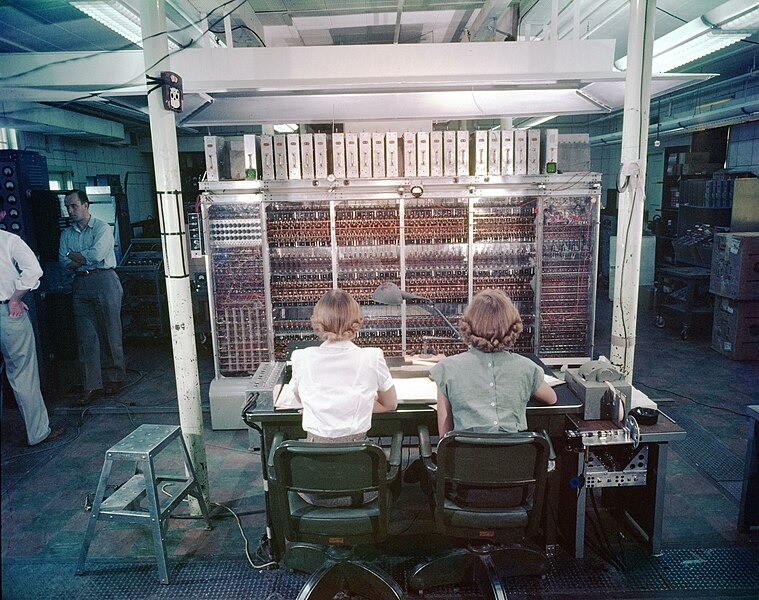
\includegraphics[width=0.4\textwidth]{Operators_in_front_of_the_MANIAC.jpg}
	\caption{MANIAC 1 one of the earliest computer.}
	\label{MANIAC}
\end{figure}

For may years this algorithm is was simply known as \textit{Metropolis Algorithm}, later in 1970 W.K. Hastings introduce more general version of this algorithm in his paper \textit{"Monte Carlo Sampling Methods Using Markov Chains and Their Applications"}. This generalized Metropolis algorithm is known as \textit{Metropolis-Hastings algorithm}(MH algorithm).

Suppose we want to simulate a random variables or sequence of random variable with probability mass function
\begin{equation}
	\pi(\theta) = \frac{f(\theta)}{K}
\end{equation}
where $ K $ is normalizing constant which is unknown or difficult to compute.

One way to simulate $ \pi(\theta) $ is to constant a Markov Chain that is easy to simulate and whose limiting distribution is $ \pi(\theta) $.
The \textit{Metropolis-Hastings algorithm} do exactly this. MH algorithm constant a time-reversible Markov Chain with desired limiting probabilities.

\subsection{Algorithm for Metropolis-Hastings}
\begin{enumerate}
	\item Start with any \textbf{initial state}  $ \theta_0 $ satisfying $ f(\theta) > 0 $.
	\item Using a \textbf{current state}  $ \theta $, sample \textbf{candidate state} $ \theta' $ for some \textbf{jumping distribution} $ q(\theta, \theta') = q(\theta'|\theta) $, which is the probability of jumping to $ \theta' $ provided the current state in $ \theta $.
	\item Given the candidate state $ \theta' $ calculate the \textbf{acceptance probability} $ \alpha(\theta,\theta') $ by,
	      \[
		      \alpha(\theta,\theta') =\min\left( \frac{\pi(\theta')q(\theta', \theta)}{\pi(\theta)q(\theta, \theta')}, 1\right) = \min\left( \frac{f(\theta')q(\theta', \theta)}{f(\theta)q(\theta, \theta')} , 1\right)
	      \]
      \item  Accept the candidate point with probability $ \alpha $.

\end{enumerate}
We can summarize the Metropolis-Hastings Algorithm as first computing,
\[ 
    \alpha(\theta_{t},\theta_{t+1}) = \min \left( \frac{f(\theta_{t+1})q(\theta_{t+1},\theta_t)}{ f(\theta_t) q(\theta_t,\theta_{t+1}) } \right)
\]
and then accepting the candidate point $ \theta_{t+1} $ with probability $ \alpha $. This generates a Markov Chain $ ( \theta_0,\theta_1,\ldots,\theta_t,\ldots ) $,
as the transition probabilities from $ \theta_t $ to $ \theta_{t+1} $ depends only on $ \theta_t $ and not on $ (\theta_0,\theta_1,\ldots,\theta_{t-1}) $.

\subsection{Metropolis-Hastings Algorithm as a Markov Chain}
To determine Metropolis-Hastings Sampling generates a Markov Chain whose stationary distribution is candidate distribution $ \pi(\theta) $ if the Metropolis-Hastings transition kernel,
\begin{equation}
    \label{transition-kernel}
    P(\theta_1\to \theta_2) = P(\theta_1,\theta_2) = q(\theta_1,\theta_2)\alpha(\theta_1,\theta_2) = q(\theta_1,\theta_2)\times \min\left( \frac{f(\theta')q(\theta', \theta)}{f(\theta)q(\theta, \theta')} , 1\right)
\end{equation}
 is time-reversible and satisfies 
 \[
         P(\theta_1, \theta_2) \pi(\theta_1) = P(\theta_2, \theta_1) \pi(\theta_2)
 \]
 or 
 \begin{equation}
     \label{balance-equatation}
     q(\theta_1,\theta_2)\alpha(\theta_1,\theta_2)\pi(\theta_1) = q(\theta_2,\theta_1)\alpha(\theta_2,\theta_1)\pi(\theta_2) \ \forall \theta_1, \theta_2
 \end{equation}

 For time-reversibility we choose jumping distribution $ q(\theta_1,\theta_2) $ to be irreducible and $ q(\theta_1,\theta_2) = q(\theta_2,\theta_1) $ and for \Cref{balance-equatation} we consider the cases.

\textbf{Case 1:} $ q(\theta_1,\theta_2)\pi(\theta_1) = q(\theta_1,\theta_2)\pi(\theta_1)$ 
Hence, $$ \alpha(\theta_1,\theta_2) = \alpha(\theta_1,\theta_2) = 1 $$
In this case \Cref{balance-equatation} will easily holds.

\textbf{Case 2:} $ q(\theta_1,\theta_2)\pi(\theta_1) > q(\theta_1,\theta_2)\pi(\theta_1)$.
Hence,
\[
    \alpha(\theta_1,\theta_2) = \frac{\pi(\theta_2)q(\theta_2,\theta_1)}{\pi(\theta_1)q(\theta_1,\theta_2)} \ \ \text{and} \ \ \alpha(\theta_2,\theta_1) = 1
\]
Then,

\begin{align*}
    P(\theta_1,\theta_2)\pi(\theta_1) &= q(\theta_1,\theta_2)\alpha(\theta_1,\theta_2) \pi(\theta_1) \\ 
    &= q(\theta_1,\theta_2) \frac{\pi(\theta_2)q(\theta_2,\theta_1)}{\pi(\theta_1)q(\theta_1,\theta_2)} \pi(\theta_1) \\
    &= q(\theta_2,\theta_1) \pi(\theta_1) = q(\theta_2,\theta_1) \alpha(\theta_2,\theta_1) \pi(\theta_1) \\ 
    &= P(\theta_2,\theta_1) \pi(\theta_2)
\end{align*}
Hence this case satisfies \Cref{balance-equatation}.

\textbf{Case 3:} $ q(\theta_1,\theta_2)\pi(\theta_1) < q(\theta_1,\theta_2)\pi(\theta_1)$
Hence,
\[
 \alpha(\theta_1,\theta_2) = 1  \ \ \text{and} \ \  \alpha(\theta_2,\theta_1) = \frac{\pi(\theta_1)q(\theta_1,\theta_2)}{\pi(\theta_2)q(\theta_2,\theta_1)} 
\]
Then,
\begin{align*}
    P(\theta_2,\theta_1)\pi(\theta_2) &= q(\theta_2,\theta_1)\alpha(\theta_2,\theta_1)\pi(\theta_2) \\ 
                                      &= q(\theta_2,\theta_1) \frac{\pi(\theta_1)q(\theta_1,\theta_2)}{\pi(\theta_2)q(\theta_2,\theta_1)} \pi(\theta_2) \\ 
                                      &= q(\theta_1,\theta_2) \pi(\theta_1) = q(\theta_1,\theta_2) \alpha(\theta_1,\theta_2) \pi(\theta_1) \\ 
                                      &=P(\theta_1,\theta_2) \pi(\theta_1)
\end{align*}
Hence also for this case \Cref{balance-equatation} is satisfied.

\subsection{Burn-In period}
A main problem with the successful implementation of Metropolis-Hastings Algorithm infect any for any MCMC Methods is number of steps until the chain approaches stationarity.
Typically the first $ 25\% $ samples are thrown out. These are called burn-in of a sample.

The name "burn-in" comes form electronics. Many electronics components fail quickly, those that don't are more reliable subset. So a burn-in is done at the factory to eliminate the worst.

There is no rule how may samples are choose as burn-in, this is vary difficult problem to answer. A poor choice of initial values and/or jumping distribution can greatly increase the requirement of burn-in time, this a hot research topic how do we choose an optimal starting point and jumping distribution. For simplicity, we choose starting value to be as close as center of the candidate distribution. 

\textbf{"Burn-in is only one method, and not a particularly good method, of finding a good starting point"}

A chain is said to be \textbf{poorly mixing} if it says in small regions of the parameter
space for long periods of time, as opposed to a well \textbf{mixing chain} that seems to
happily explore the space. A poorly mixing chain can arise because the target
distribution is multimodal and our choice of starting values traps us near one of the modes. 
To avoid this issue we can use multiple highly dispersed initial values to start several different chains.

\subsection{Choosing Jumping Distribution}
Now the question arise how to choose a best jumping distribution that works? 
There are two approaches. First and must common one is the new value $ \theta_{t+1} $ equals the current value $ \theta_t $ plus a random noise $ z $. That is,
\[
    \theta_{t+1} = \theta_t + z
\]
In this case, $ q(\theta_{t},\theta_{t+1}) = g(\Theta_{t+1}-\theta_t) = g(z) $, the density associated with the random noise $ z $. If $ g(z) = g(-z) $, i.e., the density for the random variable $ z $ is symmetric.

Typically we take, $ z $ to be from normal or multivariate normal distribution with mean zero. Then, $ \theta_{t+1} $ is form normal or multivariate normal distribution with mean $ \theta_t $. 

Then, we can use Metropolis-Hastings sampling as,
\[
    \frac{q(\theta_t,\theta_{t+1})\pi(\theta_t)}{q(\theta_{t+1},\theta_{t})\pi(\theta_{t+1})}  = \frac{g(z)\pi(\theta_t)}{g(-z)\pi(\theta_{t+1})} = \frac{\pi(\theta_t)}{\pi(\theta_{t+1})}
\]
We can adjust the variance of jumping distribution to get better mixing.

Second one is, we use an independent chain. The probability of jumping to a point $ \theta_{t+1} $ is independent of current position $ \theta_t $ of the chain, i.e. $ q(\theta_t,\theta_{t+1}) = g(y) $. Thus the current value is simply drawn from a distribution of interest, independent of current position.

\subsection{Convergence Diagnostics}
Now we have to ensure that Markov Chains have reached stationarity and only use those samples that have been generated after stationarity has been reached. But it is impossible to ensure when those two conditions are satisfied since the Markov Chain does not begin with stationary distribution. Instead we can use various methods to assess whether or not stationarity appears to have reached. Most common one is:

\textbf{Visual inspection} where we plot variable of interest vs iteration number, plot running means of variables of interest etc or run various iteration of samples with different initial states and different jumping distribution and compare them. This method is manual and need lot of works.

Another one is \textbf{Geweke test}, splits sample (after burn-in period) into two parts.
Say the first 10\% and last 50\%. If the chain is at stationarity, the means of two samples should be equal. A modified z-test can be used to comparer the two subsamples,
and the resulting test statistic is often referred to as a \textbf{Geweke z-score}.
A value larger than 2 indicates that the mean of
the series is still drifting, and a longer burn-in is required before monitoring the
chain (to extract a sampler) can begin. Formula for Geweke z-score is given by,
\[
    z = \frac{\Bar{X_1} - \Bar{X_2}}{\sqrt{ \text{Var}(X_1) + \text{Var}(X_2) }}
\]
Where, $ X_1 $ is the first 10\% subsamples and $ X_2 $ last 50\% subsamples.

\subsection{Examples}

Now we see some examples how we can use Metropolis-Hastings Algorithm. 

\begin{example}[Simulating from an unknown distribution]
    The besis problem Metropolis-Hastings algorithm solves is to provided a method for sampling from some arbitrary probability distribution. In this example we see how it is works,

    Suppose, we have 
    \[
        p(x) = \frac{e^{(-x^2)} \left( 2 + \sin(5x) + \sin(2x) \right) }{ \int_{-\infty}^{\infty} e^{(-u^2)} \left( 2 + \sin(5u) + \sin(2u) \right) du }
    \]
    Now we want to generate a random variables form $ p(x) $. It is may very hard to calculate the integration in the denominator or we don't want to calculate it. i.e., we the the probability distribution up to normalizing constant.
    So we have,
    \[
        p(x) \propto e^{(-x^2)} \left( 2 + \sin(5x) + \sin(2x) \right) 
    \]
    \begin{figure}[H]
        \centering
        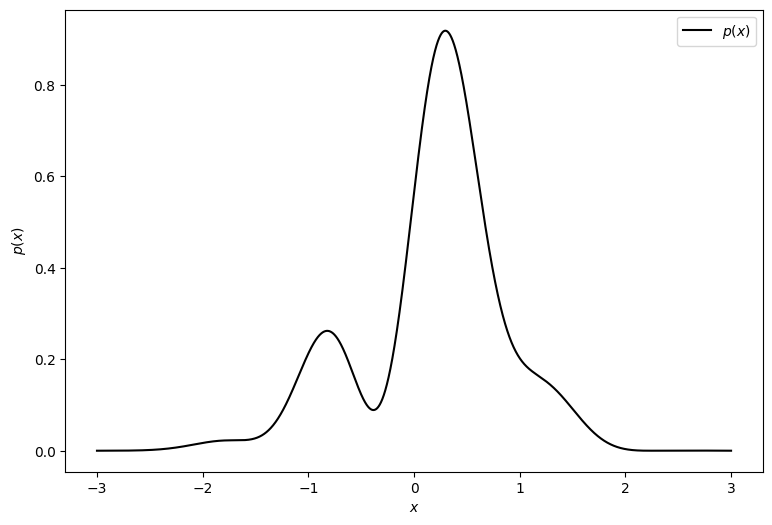
\includegraphics[width=0.6\textwidth]{./images/metropolis/plot-of-px.png}
        \caption{Plot of original $p(x)$}
        \label{plot of px}
    \end{figure}
    
\end{example}






\section{The Gibbs Sampler}

The Metropolis-Hastings Algorithm of the previous section can be difficult to apply when the dimension of the state space is high. 
The generation of the chain becomes too much of a multidimensional problem and becomes at least unwieldy, and possibly undoable.
Here Gibbs Sampler comes into play. The Gibbs Sampler is a spatial kind of Metropolis-Hastings Algorithm that very cleverly reduces the multidimensional problem into a sequence of \textit{one-dimensional} problem. 

Suppose a state $ \mathbf{x} $ in the state specs $ S $ is a vector in some $ m $-dimensional specs with $ \mathbf{x} = (x_1,x_2,x_3,\ldots,x_m) $. Suppose from current state $ \mathbf{x} $ we want to jump to a new state $ \mathbf{y}\in S $. According to Gibbs sampler we change coordinate one at a time,
such as $ (x_1,x_2,\ldots,x_m) \to (y_1,x_2,\ldots,x_m) \to (y_1,y_2,\ldots,x_m) \to \ldots \to (y_1,y_2,\ldots,y_m)  $, and each coordinate change is made by using the conditional distribution of that coordinate given the rest of the coordinates. 
For example, the transition $ (x_1,x_2,\ldots,x_m) \to (y_1,x_1,\ldots,x_m) $ is made by simulating from the distribution $ f(x_1|x_2,\ldots,x_m) $.
These conditional distribution of one coordinate gives all the rest are \textbf{full conditionals}. As, long as we can calculate and also simulate from all the full conditionals, a complicated multidimensional problem turns in to $ m $ one dimensional problems.

If current state $ \mathbf{x} = (x_1,x_2,x_3,\ldots,x_m)  $.Pick the coordinate to be changed at random from the $ m $ available coordinate. If the coordinate picked is $ i $, then the state $ \mathbf{y} = (x_1,x_2, \ldots , x_{j-1}, x , x_{j+1}, \ldots , x_m) $ work as a candidate state.
Then Gibbs sampler uses the Metropolis-Hastings algorithm with
\begin{align*}
    q(\mathbf{x},\mathbf{y}) &= \frac{1}{m} P( X_i = x | X_j = x_j, i\neq j )\\ 
                             &= \frac{f(\mathbf(y))}{mP(X_j = x_j, i \neq j)}
\end{align*}
Now the acceptance probability
\begin{align*}
    \alpha(\mathbf{x},\mathbf{y}) &= \min \left( \frac{f(\mathbf{y})q(\mathbf{y},\mathbf{x})}{f(\mathbf{x})q(\mathbf{x},\mathbf{y})} , 1 \right) \\ 
                                  &= \min \left(  \frac{ f(\mathbf{y})f(\mathbf{x}) }{  f(\mathbf{x})f(\mathbf{y})  } , 1  \right) \\ 
                                  &= 1
\end{align*}

Hence, Gibbs sampler is a special Metropolis-Hastings algorithm whose acceptance probability is always 1.

\subsection{Algorithm for Gibbs Sampler}
Suppose $ \mathbf{x}\in \mathds{R}^m $. Then algorithm of The Gibbs sampler can summarized as below:
\begin{enumerate}
    \item Set initial values $ \mathbf{x}^{(0)} = ( x_1^{(0)}, x_2^{(0)} , \ldots , x_m^{(0)}  ) $.
    \item Obtain a new value $ \mathbf{x}^{(j)} = ( x_1^{(j)}, x_2^{(j)}, \ldots , x_m^{(j)} )$ form $ x^{(j-1)} $ through \textit{full conditional distributions}
            \begin{align*}
                x_1^{(j)} &\sim f(x_1|x_2^{(j-1)}, \ldots, x_m^{(j-1)}  ),\\
                x_2^{(j)} &\sim f(x_2|x_1^{(j)}, x_3^{(j-1)}, \ldots, x_m^{(j-1)}), \\
                \vdots \\
                x_m^{(j)} &\sim f(x_m|x_1^{(j)}, \ldots , x_{m-1}^{(j)}  );
            \end{align*}
            \item Change counter $ j $ to $ j + 1 $ and return to step 2 until convergence is reached. 
\end{enumerate}

\subsection{Examples}
Now, we see some examples how to use Gibbs sampler.

\begin{example}[Generating standard bivariate normal distribution]

    In this example we try to generate standard bivariate normal distribution with correlation coefficient $ \rho $. Suppose,
    \[
        (X_1, X_2) \sim \text{N}\left(  
            \begin{bmatrix}
                0\\
                0
            \end{bmatrix},
            \begin{bmatrix}
                1 & \rho \\ 
                \rho & 1
            \end{bmatrix}
        \right)
    \]
    Where, $ \Sigma = \begin{bmatrix}
        1 & \rho \\ 
        \rho & 1
    \end{bmatrix} $ is known as \textbf{covariance matrix}.  Then, the probability density function of $ (X_1,X_2) $ would be,

    \[
        f(x_1,x_2) = \frac{1}{2 \pi \sqrt{1-\rho^2}} \exp \left( - \frac{1}{2(1-\rho^2)} (x^2 -2 \rho xy + y^2  ) \right)
    \]
    
    \begin{figure}[H]
        \centering
        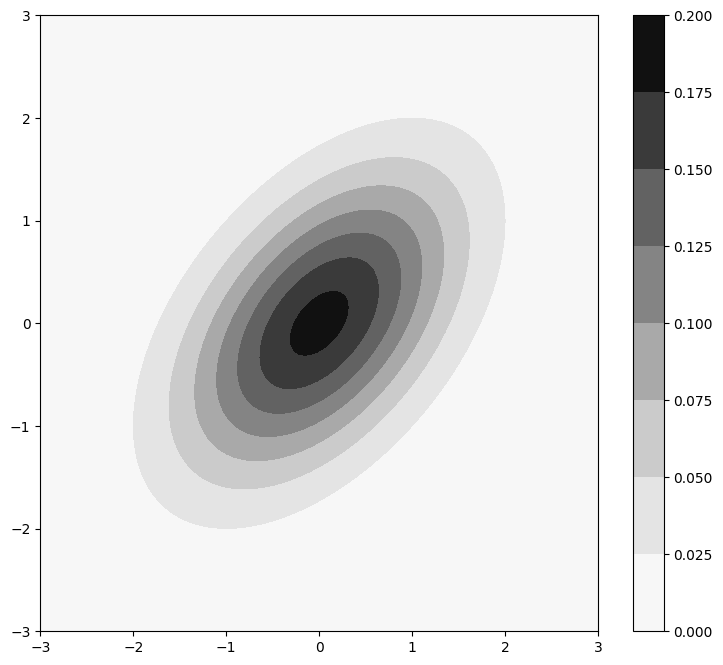
\includegraphics[width=0.6\textwidth]{images/gibbs/ex1-con-plot.png}
        \caption{Contour Plot of Bivariate Normal Distribution when $ \rho = 0.5 $}
    \end{figure}

    For using Gibbs Sampler we have to calculate $ f_{X_1|X_2}(x_1|x_2) $ and $ f_{X_2|X_1}(x_2|x_1) $.

    \begin{align*}
        f_{X_1|X_2}(x_1|x_2) &= \frac{f(x_1,x_2)}{f_{X_2}(X_2)} \\ 
                    &=C_1 f(x_1,x_2) \\
                    &=C_2 \exp \left( - \frac{1}{2 \sqrt{1-\rho^2}} (x_1^2 - 2 \rho x_1x_2) \right) \\
                    &= C_3 \exp \left(- \frac{1}{2 \sqrt{1-\rho^2}} (x_1 - \rho x_2)^2   \right)
    \end{align*}
     Recognizing this equation as a normal density, we can conclude that, 
     \[ X_1|X_2 \sim \text{N}(\rho x_2, (1-\rho^2)) \]

    Also, 
    \begin{align*}
        f_{X_2|X_1} (x_2|x_1) &= \frac{f(x_2,x_1)}{f_{X_1}(X_1)} \\ 
                    &=C_4 f(x_2,x_1) \\
                    &=C_5 \exp \left( - \frac{1}{2 \sqrt{1-\rho^2}} (x_2^2 - 2 \rho x_1x_2) \right) \\
                    &= C_6 \exp \left(- \frac{1}{2 \sqrt{1-\rho^2}} (x_2 - \rho x_1)^2   \right)
    \end{align*}
    Here also we can see that,
    \[
        X_2|X_1 \sim \text{N}\left(\rho x_1, (1-\rho^2)\right)
    \]

    So, the Gibbs sampler algorithm for this case would be,
    \begin{enumerate}
        \item Set an initial state $ \left(x_1^{(0)} , x_2^{(0)} \right) $
        \item We obtain the next state $ \left( x_1^{(t+1)} , x_2^{t+1} \right) $ through the full conditional distributions, 
            \begin{align*}
                x_1^{(t+1)} &\sim \text{N}\left(\rho x_2^{(t)}, (1-\rho^2) \right) \\
                x_2 ^{(t+1)} &\sim \text{N}\left(\rho x_1^{(t+1)}, (1-\rho^2) \right) 
            \end{align*}
    \end{enumerate}
    New we choosing different initial state we study the outputs.

    \textbf{Initial State 1:} Here we are taking initial state to be $(-1,-1)$. 
    \begin{figure}[H]
        \centering
        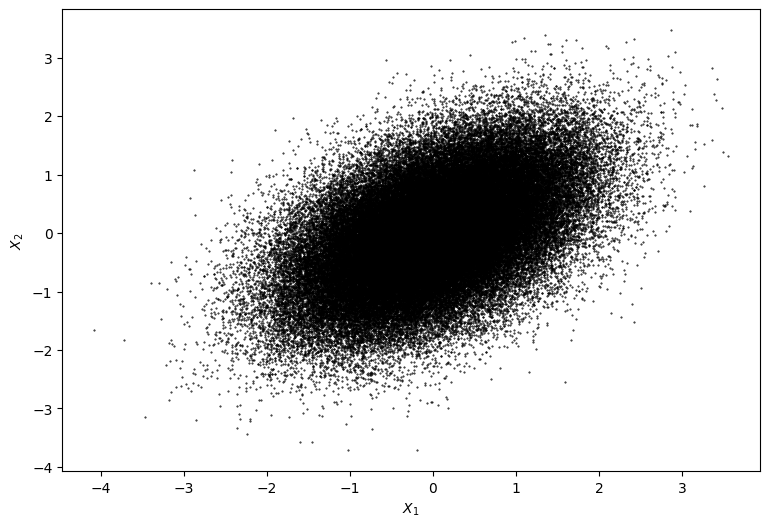
\includegraphics[width=0.5\textwidth]{images/gibbs/ex1-init1.png}
        \caption{Samples when initial state $(-1,-1)$}
    \end{figure}

    \textbf{Initial State 2:} Now we consider $(0,0)$ (middle of density) as a initial state. 

    \begin{figure}[H]
        \centering
        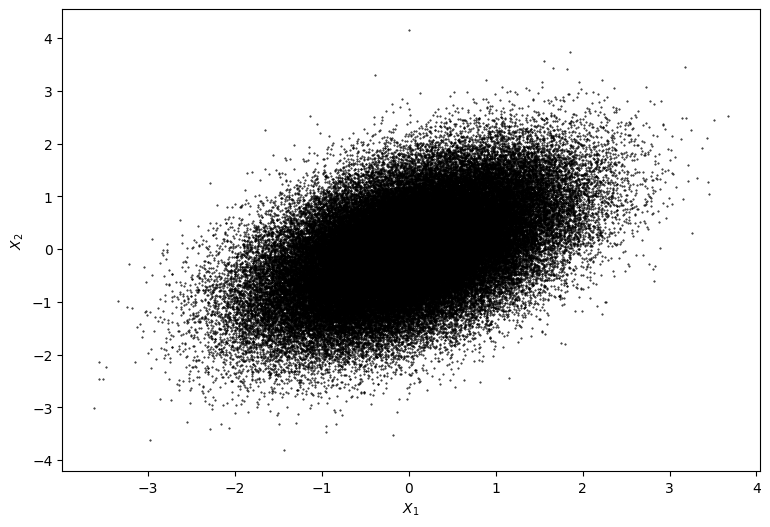
\includegraphics[width=0.5\textwidth]{images/gibbs/ex1-init2.png}
        \caption{Samples when initial state $(0,0)$}
    \end{figure}

    \textbf{Initial State 3:} Here we take initial state way out side form middle of distribution consider $ (-4,-4) $ as initial state. We can see from \Cref{fig:gb ex1 sample 3} although we are taking initial state way outside but the samples are come out to be same as above samples. 


    \begin{figure}[H]
        \centering
        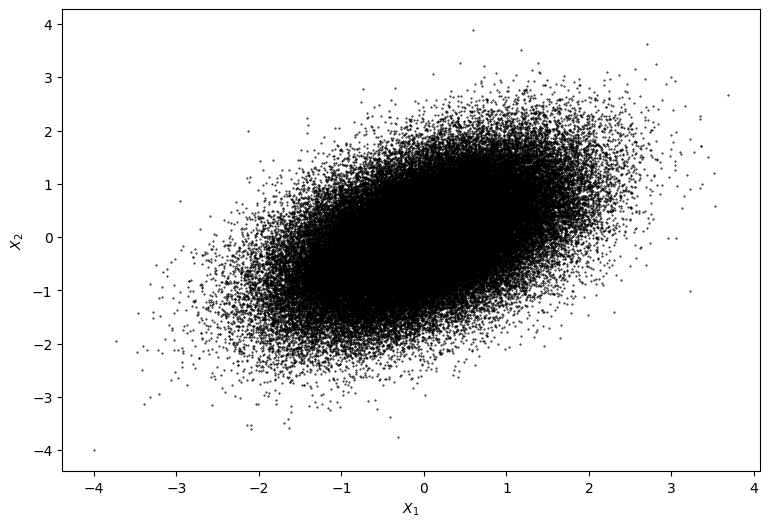
\includegraphics[width=0.5\textwidth]{images/gibbs/ex1-init3.png}
        \caption{Samples when initial state $(-4,-4)$}
        \label{fig:gb ex1 sample 3}
    \end{figure}

    \begin{figure}[H]
        \centering
        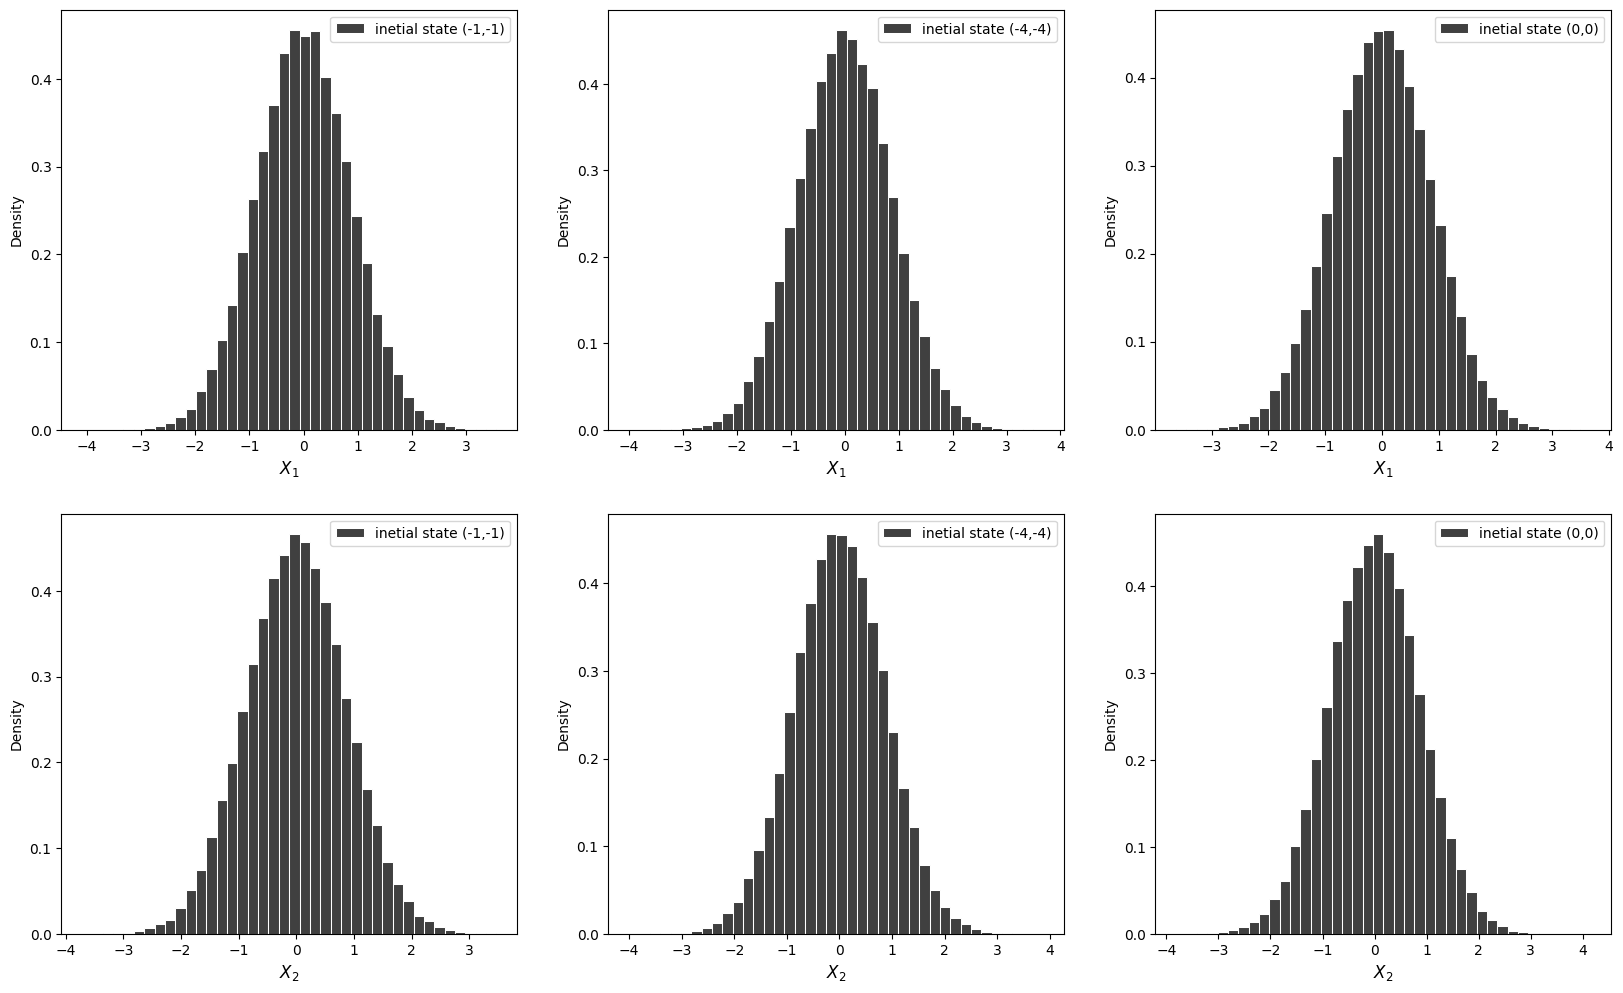
\includegraphics[width=1\textwidth]{images/gibbs/ex1-marginal-distributions.png}
        \caption{Marginal distribution for $ X_1 $ and $ X_2 $ for different initial states}
    \end{figure}

\end{example}

\begin{example}[Simulating Beta-Binomial Distribution]

    If $ X|p \sim \text{Bin}(n,p)$ for some fix $ n $, and $ p \sim \text{Beta}(\alpha,\beta) $, then the marginal distribution of $ X $ would be called a \textbf{Beta-Binomial distribution}.
    Its probability density function,
    \begin{align*}
        f_X(x) = \frac{\Gamma(\alpha+\beta)}{\Gamma(\alpha)\Gamma(\beta)} {n\choose x} \int_{0}^{1} p^{x + \alpha -1}(1-p)^{n - x + \beta -1}dp \ \ x = 0,1,2,\ldots,n  
    \end{align*}

    For simulating Beta-Binomial distribution using Gibbs sampler we have to simulate the pair $ (X,p) $ whose joint distribution is,
    \[
       f_{(X,p)}(x,p) = \frac{\Gamma(\alpha+\beta)}{\Gamma(\alpha)\Gamma(\beta)} {n\choose x} p^{x + \alpha -1}(1-p)^{n - x + \beta -1} , \, x = 0,1,2,\ldots,n, \, 0<p<1.  
    \]
    
    We know form definition of Beta-Binomial distribution,
    \[
        X|p \sim \text{Bin}(n,p)
    \]

    Now,
    \begin{align*}
        f_{p|X}(p|x) &= \frac{f(x,p)}{f(x)} \\ 
                &= \frac{ \frac{\Gamma(\alpha+\beta)}{\Gamma(\alpha)\Gamma(\beta)} {n\choose x} p^{x + \alpha -1}(1-p)^{n - x + \beta -1} }{ \frac{\Gamma(\alpha+\beta)}{\Gamma(\alpha)\Gamma(\beta)} {n\choose x} \int_{0}^{1} p^{x + \alpha -1}(1-p)^{n - x + \beta -1}dp } \\
                &= \frac{ p^{x + \alpha -1}(1-p)^{n - x + \beta -1} }{ \int_{0}^{1} p^{x + \alpha -1}(1-p)^{n - x + \beta -1}dp } \\
                &= \frac{ 1 }{ \text{Beta}(x+\alpha-1,n-x+\beta-1) } p^{x + \alpha -1}(1-p)^{n - x + \beta -1}
    \end{align*}
    Hence we have,
    \begin{equation}
        \label{eq:p|x}
        f_{p|X}(p|x) = \frac{\Gamma(\alpha+\beta+n)}{\Gamma(x+\alpha)\Gamma(n-x+\beta)} p^{x + \alpha -1}(1-p)^{n - x + \beta -1}
    \end{equation}

    Form \Cref{eq:p|x} we conclude that $ p|X\sim \text{Beta}(x+\alpha,n-x+\beta) $.

    So, the Gibbs sampler algorithm for this example,
    \begin{enumerate}
        \item Choose an initial state $ p^{(0)} \sim \text{Beta}(\alpha,\beta)  $.
        \item Obtain the next state $ \left(x^{(t+1)}, p^{(t+1)}\right) $ through the full conditional distributions,
            \begin{align*}
                x^{(t+1)} &\sim \text{Bin}\left( n,p^{(t)} \right),\\
                p^{(t+1)} &\sim \text{Beta}\left(x^{(t+1)}+\alpha, n-x^{(t+1)}+\beta \right) 
            \end{align*}
        \item Replete step 2.  
    \end{enumerate}

    Now, taking $ n=10,\,\alpha=7,\,\beta=2 $ we simulate beta-binomial distribution and we get empirical mean 7.7797, variance 3.2788 which are close to theoretical mean($ \mu $) and variance($ \sigma^2 $).
    \begin{align*}
        \mu &= \frac{n \alpha}{\alpha+\beta} = \frac{10 \times 7 }{ 7 + 2} = 7.7777 \\
        \sigma^2 &= \frac{n \alpha \beta(\alpha+\beta+n)}{(\alpha+\beta)^2(\alpha+\beta+1)} = 3.2840
    \end{align*}
    
    \begin{figure}[H]
        \centering
        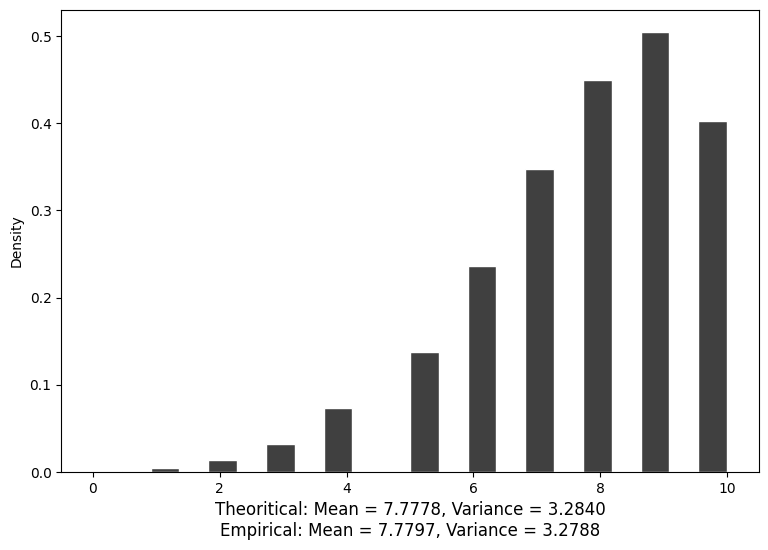
\includegraphics[width=0.6\textwidth]{images/gibbs/ex2-beta-binomial.png}
        \caption{Simulation of Beta-Binomial(10,7,2)}
        \label{fig:beta-binomial simulation}
    \end{figure}

\end{example}

\begin{example}[Finding distribution of some observed data]
    In the \Cref{eg:finding parameter} we have done a little cheating, here we did not find the mean($\mu$) in proper way, we assume the mean from the given observation, but this is not the proper way.  In this example we try to fix our mistake. 

    Now, from \textbf{Bayesian Method} we have
    \begin{equation}
        \label{eq:proper bayesian formula}
        f\left(\mu, \sigma^2|d^{n} \right) \propto f\left( d^{n} |\mu,\sigma^2 \right) f\left( \mu,\sigma^2 \right)
    \end{equation}

    The \textbf{likelihood function},
    \begin{align*}
        f\left( d^{n} |\mu,\sigma^2 \right) &= \prod_{i=1}^{n} \left( \frac{1}{\sqrt{2 \pi \sigma^2 }} \exp \left( - \frac{ (d_i - \mu)^2 }{ 2 \sigma^2 } \right) \right) \\ 
                                            &= \frac{ 1 }{ \left( 2 \pi \sigma^{2}  \right)^{\frac{n}{2}}  } \exp \left( - \frac{ \sum_{i = 1}^{n} \left( d_i - \mu \right)^{2}   }{ 2 \sigma^2 } \right) \numberthis \label{eq:likelihood function}
    \end{align*}
    
    Then \Cref{eq:proper bayesian formula} becomes, 
    \begin{equation}
         \label{eq:full equatation of proper bayesian formula}
         f(\mu,\sigma^{2} |d^{n} ) \propto \frac{ 1 }{ \left( 2 \pi \sigma^{2}  \right)^{\frac{n}{2}}  } \exp \left( - \frac{ \sum_{i = 1}^{n} \left( d_i - \mu \right)^{2}   }{ 2 \sigma^2 } \right) f(\mu,\sigma^2)
     \end{equation}

     Then, the question become how do we choose the \textbf{prior} in this case. We can consider the two possibilities,
     \begin{enumerate}
         \item We can define a joint prior distribution for $ \mu $ and $ \sigma^{2}  $, i.e. we can define $ f(\mu,\sigma^{2} ) $, but it will very hard to accomplish. 
         \item Another way we can consider $ \mu $ and $ \sigma^{2}  $ to be independent. i.e., 
             \[ f(\mu, \sigma^{2} ) = f_\mu(\mu)f_{\sigma^{2} } (\sigma^{2})  \] 
             This is relatively easy to implement.
     \end{enumerate}

     Here if we take \fdefine{conjugate prior}{In Bayesian Inference, for a given likelihood function $ f(x|\theta) $, if the posterior distribution $ f(\theta|x) $ is in the same probability density family as the prior $ f(\theta) $, then the prior and posterior are called conjugate distributions with respect to that likelihood function and the prior is called a conjugate prior for the likelihood function $ f(x|\theta) $. } as our choice of prior it will be easy to sample from posterior distribution.

     Now we have the conjugate prior for $ \mu $ for normal likelihood function is Normal distribution.
     \begin{align*}
         f_{\mu} (\mu) &\propto \tx{N}\left( \theta,\sigma_{\mu}^{2}  \right) \\
                       &\propto \frac{ 1 }{ \sqrt{2 \pi \sigma_{\mu} ^{2} } } \exp \left( - \frac{ (\mu - \theta)^{2} }{ 2 \sigma_{\mu} ^{2}  } \right)
     \end{align*}
     Where, $ \theta $ and $ \sigma_{\mu}^{2} $ are \textbf{hyperparameters} of the prior distribution. 

     And for $ \sigma^2 $ we have two choices for conjugate prior for normal likelihood function.
     \begin{enumerate}
         \item One is Inverse-gamma distribution.
             \begin{align*}
                 f_{\sigma^2}(\sigma ^{2}) &\propto \tx{Inv-Gamma}(\alpha,\beta) \\
                              &\propto \frac{ \beta^{\alpha}  }{ \Gamma(\alpha) } \left( \frac{ 1 }{ \sigma^2 } \right)^{(\alpha+1)} \exp \left( - \frac{ \beta }{ \sigma ^{2}  } \right)
             \end{align*}

             with \textbf{hyperparameters} $ \alpha > 0 $, shape\footnote{shape parameters are those parameter those effect the shape of the distribution} parameter of $ f_{\sigma ^{2}}(\sigma ^{2})  $ and $ \beta > 0 $, scale \footnote{ In family of probability distribution there is such parameter $ s $(with other parameter $ \theta $) for which the CDF satisfies $F(x;s,\theta) = F(x/s;1,\theta)$ known as scale parameter} parameter of $ f_{\sigma ^{2}}(\sigma ^{2})  $

        \item Another one is Scaled-Inverse-$\chi ^{2}$ distribution.
            \begin{align*}
                f_{\sigma ^{2} }(\sigma ^{2}) &\propto \tx{Scale-Inv-}\chi^2\left( \nu,\sigma ^{2}_0 \right)\\ 
                                              &\propto \frac{ \left( \sigma_{0}^{2}\nu/2 \right)^{\nu/2}   }{ \Gamma(\nu/2) } \frac{ \exp\left( - \frac{ \nu \sigma_0 ^{2} }{ 2 \sigma ^{2} } \right) }{ \left( \sigma^2 \right)^{1+\nu/2}  }
            \end{align*}
            With hyperparameters $ \nu $ and $ \sigma_0 ^{2} $.
     \end{enumerate}

     Now, if we choose prior of $ \sigma ^{2} $ to be Inv-Gamma$(\alpha,\beta)$ and $ \mu $ to be N$(\theta,\sigma_{\mu}^{2} )$ \Cref{eq:full equatation of proper bayesian formula} becomes,

    \begin{align*}
        f(\mu,\sigma ^{2}|d ^{n} ) \propto &\frac{ 1 }{ \left( 2 \pi \sigma^{2}  \right)^{\frac{n}{2}}  } \exp \left( - \frac{ \sum_{i = 1}^{n} \left( d_i - \mu \right)^{2}   }{ 2 \sigma^2 } \right) \times \\
        &\frac{ 1 }{ \sqrt{2 \pi \sigma_{\mu} ^{2} } } \exp \left( - \frac{ (\mu - \theta)^{2} }{ 2 \sigma_{\mu} ^{2}  } \right) \times \left( \frac{ 1 }{ \sigma^2 } \right)^{(\alpha+1)} \exp \left( - \frac{ \beta }{ \sigma ^{2}  } \right) \numberthis \label{eq:posterior imposible to calculate}
    \end{align*}

    For simulating \Cref{eq:posterior imposible to calculate} we will use Gibbs sampler. To use Gibbs sampler we have to find the full conditionals $ f(\mu|d^{n},\sigma^2 ) $ and $ f(\sigma^{2}|d^{n}, \mu) $.
    
    Now, 
    \begin{align*}
        f(\mu|d^{n},\sigma^{2} ) &\propto \exp \left( - \frac{ \sum_{i = 1}^{n}(d_i - \mu)^2  }{ 2 \sigma^{2} } \right) \times \exp \left( - \frac{ (\mu-\theta)^{2} }{ 2 \sigma_{\mu} ^{2} } \right) \\ 
                                 &\propto \exp \left( - \frac{ 1 }{ 2 } \left( \frac{ \sum_{i = 1}^{n}(d_i - \mu)^2  }{ \sigma^{2} } + \frac{ (\mu-\theta)^{2} }{ \sigma_{\mu} ^{2} } \right) \right) \\ 
                                 &\propto \exp \left( - \frac{ 1 }{ 2 } \left( \frac{ \sum_{i=1}^{n} d_i^{2} - 2 \mu \sum_{i=1}^{n} d_i + n \mu^{2} }{ \sigma^{2} } + \frac{ \mu^{2} - 2 \mu \theta + \theta^{2} }{ \sigma_\mu^{2} }  \right) \right) \\ 
                                 &\propto \exp \left( - \frac{ 1 }{ 2 } \left( \frac{ \sigma_\mu^{2} \sum_{i=1}^{n} d_i^{2} - 2 \sigma_\mu^{2} \mu \sum_{i=1}^{n} d_i + \sigma_\mu^{2} n \mu^{2} + \sigma^{2}\mu^{2} - 2 \sigma^{2}\mu \theta + \sigma^{2}\theta^{2} }{ \sigma^{2}\sigma_\mu^{2} } \right) \right) \\
                                 &\propto \exp \left( - \frac{ 1 }{ 2 }  \frac{ \left( n \sigma_{\mu}^{2} + \sigma^{2}  \right)\mu^{2} - 2 \mu \left( \sigma_{\mu}^{2}\sum_{i=1}^{n}d_i + \sigma^{2}\theta  \right)   }{ \sigma^{2}\sigma_{\mu} ^{2} } \right) \\
                                 &\propto \exp \left( - \frac{ 1 }{ 2 } \frac{ \mu^{2} - 2 \mu \left( \frac{ \sigma_{\mu}^{2}\sum_{i=1}^{n} d_i + \sigma^{2}\theta  }{ n \sigma_{\mu}^{2} + \sigma^{2}  } \right) }{ \frac{ \sigma_{\mu}^{2}\sigma^{2} }{  n \sigma_{\mu}^{2} + \sigma^{2} } }  \right) \\
                                 &\propto \exp \left( - \frac{ \left( \mu - \frac{ \sigma_{\mu}^{2}\sum_{i=1}^{n} d_i + \sigma^{2}\theta }{ n \sigma_{\mu}^{2}+\sigma^{2}  } \right)^{2} }{ 2 \left( \frac{ \sigma^{2}\sigma_{\mu}^{2}  }{  n \sigma_{\mu}^{2}+\sigma^{2} } \right) } \right) \\ 
                                 &\propto \tx{N}\left( \frac{ \sigma_{\mu}^{2}\sum_{i=1}^{n} d_i + \sigma^{2}\theta  }{ n \sigma_{\mu}^{2} + \sigma^{2} }, \frac{ \sigma_{\mu}^{2}\sigma^{2}  }{ n \sigma_{\mu}^{2} + \sigma^{2} } \right)
    \end{align*}
    So, posterior of $ \mu $ is a normal distribution with,
    \begin{align*}
        \tx{mean }= \frac{ \sigma_{\mu}^{2}\sum_{i=1}^{n} d_i + \sigma^{2}\theta  }{ n \sigma_{\mu}^{2} + \sigma^{2} }\, \tx{ and  variance }= \frac{ \sigma_{\mu}^{2}\sigma^{2}  }{ n \sigma_{\mu}^{2} + \sigma^{2} }
    \end{align*}

    Now if we take Inv-Gamma as prior of $ \sigma^{2} $ we get,
    \begin{align*}
        f(\sigma^{2}|d^{n} \mu) &\propto \left(\frac{ 1 }{\sigma^{2}}\right)^{\frac{ n }{2}} \exp \left( - \frac{ \sum_{i=1}^{n} (d_i - \mu)^{2} }{ 2 \sigma^{2} } \right) 
        \left( \frac{ 1 }{ \sigma^{2} }\right)^{\alpha+1}  \exp \left( - \frac{ \beta }{ \sigma^{2}  } \right) \\ 
                                &\propto \left( \frac{ 1 }{ \sigma^{2} } \right)^{\alpha + \frac{ n }{ 2 } + 1} 
                                \exp \left( - \frac{ 2\beta + \sum_{i=1}^{n} (d_i-\mu)^{2} }{ 2\sigma^{2} } \right) \\ 
                                &\propto \left( \frac{ 1 }{ \sigma^{2} } \right)^{\alpha + \frac{ n }{ 2 } + 1}
                                \exp \left( - \frac{ \beta + \frac{ \sum_{i=1}^{n} (d_i-\mu)^{2} }{ 2 } }{ \sigma^{2} } \right) \\ 
                                &\propto \tx{Inv-Gamma}\left( \alpha + \frac{ n }{ 2 }, \beta + \frac{ \sum_{i=1}^{n} (d_i-\mu)^{2} }{ 2 } \right)
    \end{align*}

    And now if we take Scale-Inv-$ \chi^{2} $ as prior of $ \sigma^{2} $ we the posterior to be,
    \begin{align*}
        f(\sigma^{2}|d^{n} ,\mu) &\propto \left( \frac{ 1 }{ 2 \pi \sigma^{2} } \right)^{n/2} 
        \exp \left( - \frac{ \sum_{i=1}^{n} (d_i - \mu)^{2} }{ 2 \sigma^{2} } \right) 
        \left( \frac{ 1 }{ \sigma^{2} } \right)^{1+\frac{ \nu }{ 2 }}
        \exp \left( - \frac{ \nu \sigma_0^{2} }{ 2 \sigma^{2} } \right) \\ 
                                 &\propto \left( \frac{ 1 }{ \sigma^{2} } \right)^{1+\frac{ \nu+ n }{ 2 }} 
        \exp \left( - \frac{ \sum_{i=1}^{n}(d_i-\mu)^{2} + \nu \sigma_0^{2}  }{ 2 \sigma^{2} } \right) \\ 
                                 &\propto \left( \frac{ 1 }{ \sigma^{2} } \right)^{1+\frac{ \nu+ n }{ 2 }} 
                                 \exp \left( - \frac{ (\nu + n) \frac{ \sum_{i=1}^{n}(d_i-\mu)^{2} + \nu \sigma_0^{2} }{ \nu + n } }{ 2 \sigma^{2} } \right) \\ 
                                 &\propto \tx{Scale-Inv-}\chi^{2}\left( \nu + n, \frac{ \sum_{i=1}^{n}(d_i-\mu)^{2} + \nu \sigma_0^{2} }{ \nu + n } \right)
    \end{align*}

 \end{example}





\nocite{*}
\phantomsection
\addcontentsline{toc}{chapter}{Bibliography}
\bibliographystyle{unsrt}
\bibliography{Referance}

\end{document}
